\documentclass[border=10pt]{standalone}
\usepackage{pgfplots, tikz, amsmath}
\usepackage{filecontents}

\usepgfplotslibrary{colorbrewer}
\usepgfplotslibrary{fillbetween, external}

\definecolor{blueish}{RGB}{48,140,43}

\begin{document}
\begin{tikzpicture}
  \begin{axis}[
 	ylabel={$A(t)/\pi R_o^2$},
	xlabel= $t/T$,
	width = 6cm,
	height = 4.5cm,
	xmin=0,
	xmax=1,
%	cycle list/Paired-5,
	minor tick style={draw=none}
	]
%      \addplot +[blueish, thick, mark options={fill=blueish,scale=0.05}] table[x=x,y=y] {./data/AreaAverage.txt};
      \addplot +[blueish, thick, no marks] table[x=x,y=y] {./data/AreaAverage.txt};
      \addplot [name path=upper,draw=none] table[mark options={fill=blueish,scale=1}, x=x,y expr=\thisrow{y}+\thisrow{err}] {./data/AreaAverage.txt};
      \addplot [name path=lower,draw=none] table[mark options={fill=black,scale=1}, x=x,y expr=\thisrow{y}-\thisrow{err}] {./data/AreaAverage.txt};
      \addplot [fill=black!10] fill between[of=upper and lower];

  \end{axis}
\end{tikzpicture}

%% This file was created by tikzplotlib v0.9.8.
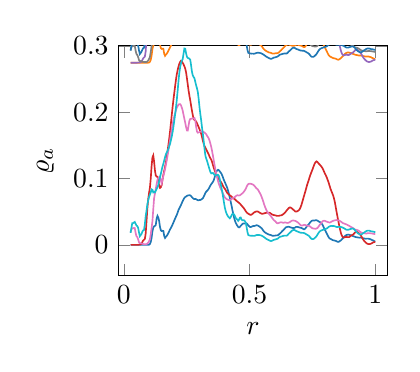
\begin{tikzpicture}

\definecolor{color0}{rgb}{0.12156862745098,0.466666666666667,0.705882352941177}
\definecolor{color1}{rgb}{1,0.498039215686275,0.0549019607843137}
\definecolor{color2}{rgb}{0.172549019607843,0.627450980392157,0.172549019607843}
\definecolor{color3}{rgb}{0.83921568627451,0.152941176470588,0.156862745098039}
\definecolor{color4}{rgb}{0.580392156862745,0.403921568627451,0.741176470588235}
\definecolor{color5}{rgb}{0.549019607843137,0.337254901960784,0.294117647058824}
\definecolor{color6}{rgb}{0.890196078431372,0.466666666666667,0.76078431372549}
\definecolor{color7}{rgb}{0.737254901960784,0.741176470588235,0.133333333333333}
\definecolor{color8}{rgb}{0.0901960784313725,0.745098039215686,0.811764705882353}

\begin{axis}[
xlabel={\(\displaystyle r\)},
xmin=-0.0219063545150502, xmax=1.04866220735786,
ylabel={\(\displaystyle \varrho_a\)},
ymin=-0.0462788671023965, ymax=0.971856209150327,
width=5cm,
height=4.5cm,
ymax=0.3
]
\addplot [semithick, color0]
table {%
0 nan
0.00334448160535117 nan
0.00668896321070234 nan
0.0100334448160535 nan
0.0133779264214047 nan
0.0167224080267559 nan
0.020066889632107 nan
0.0234113712374582 nan
0.0267558528428094 0
0.0301003344481605 0
0.0334448160535117 0
0.0367892976588629 0
0.040133779264214 0
0.0434782608695652 0
0.0468227424749164 0
0.0501672240802676 0
0.0535117056856187 0
0.0568561872909699 0
0.0602006688963211 0
0.0635451505016722 0
0.0668896321070234 0
0.0702341137123746 0
0.0735785953177257 0
0.0769230769230769 0
0.0802675585284281 0
0.0836120401337793 0
0.0869565217391304 0
0.0903010033444816 0
0.0936454849498328 0
0.096989966555184 4.35729847494529e-05
0.100334448160535 0.000305010893246182
0.103678929765886 0.00135076252723311
0.107023411371237 0.00435729847494553
0.110367892976589 0.0105010893246187
0.11371237458194 0.0203921568627451
0.117056856187291 0.0259259259259259
0.120401337792642 0.0280610021786492
0.123745819397993 0.0286274509803922
0.127090301003344 0.030239651416122
0.130434782608696 0.0396078431372549
0.133779264214047 0.0437908496732026
0.137123745819398 0.0412636165577342
0.140468227424749 0.0359912854030501
0.1438127090301 0.0269716775599129
0.147157190635451 0.0221786492374728
0.150501672240803 0.0209150326797386
0.153846153846154 0.0212636165577342
0.157190635451505 0.0210893246187364
0.160535117056856 0.0134640522875817
0.163879598662207 0.0104139433551198
0.167224080267559 0.012156862745098
0.17056856187291 0.0136383442265795
0.173913043478261 0.0154684095860566
0.177257525083612 0.017995642701525
0.180602006688963 0.0207407407407407
0.183946488294314 0.0233986928104575
0.187290969899666 0.0257516339869281
0.190635451505017 0.0281045751633987
0.193979933110368 0.0308061002178649
0.197324414715719 0.0337690631808279
0.20066889632107 0.0368191721132898
0.204013377926421 0.0397821350762527
0.207357859531773 0.0425708061002179
0.210702341137124 0.0453159041394336
0.214046822742475 0.0488453159041394
0.217391304347826 0.0524618736383442
0.220735785953177 0.0552941176470588
0.224080267558528 0.0575599128540305
0.22742474916388 0.0602614379084967
0.230769230769231 0.0631808278867102
0.234113712374582 0.0661437908496732
0.237458193979933 0.0687145969498911
0.240802675585284 0.0708061002178649
0.244147157190635 0.072156862745098
0.247491638795987 0.0729847494553377
0.250836120401338 0.0738126361655774
0.254180602006689 0.0744662309368192
0.25752508361204 0.0746840958605665
0.260869565217391 0.0749455337690632
0.264214046822742 0.074640522875817
0.267558528428094 0.0735511982570806
0.270903010033445 0.0719389978213508
0.274247491638796 0.0705446623093682
0.277591973244147 0.0694117647058824
0.280936454849498 0.0690631808278867
0.284280936454849 0.0693681917211329
0.287625418060201 0.0688453159041394
0.290969899665552 0.0680610021786492
0.294314381270903 0.0673202614379085
0.297658862876254 0.0673202614379085
0.301003344481605 0.0677124183006536
0.304347826086957 0.0677124183006536
0.307692307692308 0.0684531590413943
0.311036789297659 0.0692374727668845
0.31438127090301 0.0702832244008715
0.317725752508361 0.0726797385620915
0.321070234113712 0.0754248366013072
0.324414715719064 0.0783442265795207
0.327759197324415 0.0803050108932462
0.331103678929766 0.0814814814814815
0.334448160535117 0.082962962962963
0.337792642140468 0.0848366013071895
0.341137123745819 0.0873202614379085
0.344481605351171 0.0895860566448802
0.347826086956522 0.091677559912854
0.351170568561873 0.0932897603485839
0.354515050167224 0.0951633986928105
0.357859531772575 0.0977777777777778
0.361204013377926 0.101960784313725
0.364548494983278 0.106753812636166
0.367892976588629 0.11037037037037
0.37123745819398 0.112200435729847
0.374581939799331 0.113202614379085
0.377926421404682 0.112549019607843
0.381270903010033 0.110893246187364
0.384615384615385 0.109193899782135
0.387959866220736 0.107450980392157
0.391304347826087 0.104705882352941
0.394648829431438 0.101350762527233
0.397993311036789 0.0976906318082789
0.40133779264214 0.0949455337690632
0.404682274247492 0.0918954248366013
0.408026755852843 0.0889760348583878
0.411371237458194 0.0859694989106754
0.414715719063545 0.0815250544662309
0.418060200668896 0.0763834422657952
0.421404682274247 0.0711546840958605
0.424749163879599 0.0655773420479303
0.42809364548495 0.0596949891067538
0.431438127090301 0.0532026143790849
0.434782608695652 0.0470588235294117
0.438127090301003 0.0416122004357298
0.441471571906354 0.0369934640522876
0.444816053511706 0.0334204793028322
0.448160535117057 0.0309368191721133
0.451505016722408 0.02880174291939
0.454849498327759 0.0269281045751634
0.45819397993311 0.0263616557734205
0.461538461538462 0.0271459694989107
0.464882943143813 0.0288453159041394
0.468227424749164 0.0299782135076253
0.471571906354515 0.0315904139433551
0.474916387959866 0.0322440087145969
0.478260869565217 0.032156862745098
0.481605351170569 0.0323747276688453
0.48494983277592 0.032636165577342
0.488294314381271 0.0325054466230937
0.491638795986622 0.0312418300653594
0.494983277591973 0.0292374727668845
0.498327759197324 0.0281481481481481
0.501672240802676 0.0270152505446623
0.505016722408027 0.0270152505446623
0.508361204013378 0.0274945533769063
0.511705685618729 0.0281045751633986
0.51505016722408 0.0284967320261437
0.518394648829431 0.0284531590413943
0.521739130434783 0.0288017429193899
0.525083612040134 0.0293681917211329
0.528428093645485 0.0296296296296296
0.531772575250836 0.0293246187363834
0.535117056856187 0.0286710239651416
0.538461538461538 0.0279738562091503
0.54180602006689 0.0269281045751634
0.545150501672241 0.0260566448801743
0.548494983277592 0.024880174291939
0.551839464882943 0.0230501089324618
0.555183946488294 0.0212200435729847
0.558528428093645 0.0197821350762527
0.561872909698997 0.0187363834422658
0.565217391304348 0.0179084967320261
0.568561872909699 0.0171241830065359
0.57190635451505 0.0166013071895425
0.575250836120401 0.0158169934640523
0.578595317725752 0.0153812636165577
0.581939799331104 0.0151633986928104
0.585284280936455 0.0148583877995642
0.588628762541806 0.014161220043573
0.591973244147157 0.013681917211329
0.595317725752508 0.0137690631808279
0.598662207357859 0.0139433551198257
0.602006688963211 0.0140740740740741
0.605351170568562 0.0142919389978213
0.608695652173913 0.0143790849673202
0.612040133779264 0.0145533769063181
0.615384615384615 0.0151633986928104
0.618729096989967 0.0165141612200435
0.622073578595318 0.0176470588235294
0.625418060200669 0.0187799564270152
0.62876254180602 0.0202614379084967
0.632107023411371 0.0215250544662309
0.635451505016722 0.0227015250544662
0.638795986622074 0.0240958605664488
0.642140468227425 0.0255337690631808
0.645484949832776 0.0266230936819172
0.648829431438127 0.0269716775599128
0.652173913043478 0.0273202614379085
0.655518394648829 0.0273202614379085
0.658862876254181 0.0270588235294117
0.662207357859532 0.0265795206971677
0.665551839464883 0.0261437908496732
0.668896321070234 0.0256644880174292
0.672240802675585 0.0254901960784313
0.675585284280936 0.0254030501089324
0.678929765886288 0.0257516339869281
0.682274247491639 0.0264488017429194
0.68561872909699 0.0271023965141612
0.688963210702341 0.0271895424836601
0.692307692307692 0.0269716775599128
0.695652173913043 0.0265795206971677
0.698996655518395 0.0262309368191721
0.702341137123746 0.0258823529411764
0.705685618729097 0.0255773420479303
0.709030100334448 0.0250544662309368
0.712374581939799 0.0243137254901961
0.71571906354515 0.0235729847494553
0.719063545150502 0.0237472766884531
0.722408026755853 0.0249673202614379
0.725752508361204 0.0267102396514161
0.729096989966555 0.0284531590413943
0.732441471571906 0.0298039215686274
0.735785953177257 0.0313289760348584
0.739130434782609 0.0329847494553377
0.74247491638796 0.0344226579520697
0.745819397993311 0.0358169934640523
0.749163879598662 0.0366013071895425
0.752508361204013 0.0368627450980392
0.755852842809364 0.0368627450980392
0.759197324414716 0.0368627450980392
0.762541806020067 0.0371677559912854
0.765886287625418 0.0372549019607843
0.769230769230769 0.0367755991285403
0.77257525083612 0.0360348583877996
0.775919732441472 0.0351633986928105
0.779264214046823 0.0344662309368192
0.782608695652174 0.0338126361655773
0.785953177257525 0.032636165577342
0.789297658862876 0.0308932461873638
0.792642140468227 0.0284531590413943
0.795986622073579 0.0255773420479303
0.79933110367893 0.0230501089324619
0.802675585284281 0.0206535947712418
0.806020066889632 0.0180827886710239
0.809364548494983 0.0153376906318082
0.812709030100334 0.0127668845315904
0.816053511705686 0.0108061002178649
0.819397993311037 0.00958605664488014
0.822742474916388 0.00888888888888884
0.826086956521739 0.00827886710239648
0.82943143812709 0.00749455337690629
0.832775919732441 0.00697167755991282
0.836120401337793 0.00671023965141609
0.839464882943144 0.00644880174291936
0.842809364548495 0.0060130718954248
0.846153846153846 0.00549019607843134
0.849498327759197 0.00479302832244006
0.852842809364548 0.00453159041394333
0.8561872909699 0.00496732026143789
0.859531772575251 0.0059259259259259
0.862876254180602 0.006797385620915
0.866220735785953 0.00801742919389976
0.869565217391304 0.00941176470588233
0.872909698996655 0.010718954248366
0.876254180602007 0.0121132897603486
0.879598662207358 0.0134640522875817
0.882943143812709 0.0143790849673202
0.88628762541806 0.0149891067538126
0.889632107023411 0.0153812636165577
0.892976588628763 0.0155555555555555
0.896321070234114 0.0152069716775599
0.899665551839465 0.0148583877995642
0.903010033444816 0.014553376906318
0.906354515050167 0.0141612200435729
0.909698996655518 0.0135511982570806
0.91304347826087 0.013115468409586
0.916387959866221 0.012636165577342
0.919732441471572 0.0121132897603486
0.923076923076923 0.0117647058823529
0.926421404682274 0.0115904139433551
0.929765886287625 0.0113289760348584
0.933110367892977 0.0110239651416122
0.936454849498328 0.0108932461873638
0.939799331103679 0.0110239651416122
0.94314381270903 0.0108932461873638
0.946488294314381 0.0105882352941176
0.949832775919732 0.0101960784313725
0.953177257525084 0.00993464052287579
0.956521739130435 0.00976034858387796
0.959866220735786 0.00941176470588233
0.963210702341137 0.00936819172113287
0.966555183946488 0.00945533769063178
0.969899665551839 0.00945533769063178
0.973244147157191 0.00932461873638341
0.976588628762542 0.00901960784313721
0.979933110367893 0.00867102396514157
0.983277591973244 0.00814814814814811
0.986622073578595 0.00745098039215682
0.989966555183946 0.00697167755991282
0.993311036789298 0.00636165577342044
0.996655518394649 0.00557734204793025
1 0.00483660130718951
};
\addplot [semithick, color1]
table {%
0 nan
0.00334448160535117 nan
0.00668896321070234 nan
0.0100334448160535 nan
0.0133779264214047 nan
0.0167224080267559 nan
0.020066889632107 nan
0.0234113712374582 nan
0.0267558528428094 0.274509803921569
0.0301003344481605 0.274509803921569
0.0334448160535117 0.274509803921569
0.0367892976588629 0.274509803921569
0.040133779264214 0.274509803921569
0.0434782608695652 0.274509803921569
0.0468227424749164 0.274509803921569
0.0501672240802676 0.274509803921569
0.0535117056856187 0.274509803921569
0.0568561872909699 0.274509803921569
0.0602006688963211 0.274509803921569
0.0635451505016722 0.274509803921569
0.0668896321070234 0.274509803921569
0.0702341137123746 0.274509803921569
0.0735785953177257 0.274509803921569
0.0769230769230769 0.274509803921569
0.0802675585284281 0.274509803921569
0.0836120401337793 0.274509803921569
0.0869565217391304 0.274509803921569
0.0903010033444816 0.274509803921569
0.0936454849498328 0.274509803921569
0.096989966555184 0.274553376906318
0.100334448160535 0.274814814814815
0.103678929765886 0.275860566448802
0.107023411371237 0.278867102396514
0.110367892976589 0.285010893246187
0.11371237458194 0.294901960784314
0.117056856187291 0.300435729847495
0.120401337792642 0.302570806100218
0.123745819397993 0.303137254901961
0.127090301003344 0.304749455337691
0.130434782608696 0.314117647058824
0.133779264214047 0.318300653594771
0.137123745819398 0.315773420479303
0.140468227424749 0.310501089324619
0.1438127090301 0.301481481481482
0.147157190635451 0.296688453159041
0.150501672240803 0.295424836601307
0.153846153846154 0.295773420479303
0.157190635451505 0.295599128540305
0.160535117056856 0.28797385620915
0.163879598662207 0.284923747276689
0.167224080267559 0.286666666666667
0.17056856187291 0.288148148148148
0.173913043478261 0.289978213507625
0.177257525083612 0.292505446623094
0.180602006688963 0.295250544662309
0.183946488294314 0.297908496732026
0.187290969899666 0.300261437908497
0.190635451505017 0.302614379084967
0.193979933110368 0.305315904139434
0.197324414715719 0.308278867102397
0.20066889632107 0.311328976034858
0.204013377926421 0.314291938997821
0.207357859531773 0.317080610021787
0.210702341137124 0.319825708061002
0.214046822742475 0.323355119825708
0.217391304347826 0.326971677559913
0.220735785953177 0.329803921568627
0.224080267558528 0.332069716775599
0.22742474916388 0.334771241830065
0.230769230769231 0.337690631808279
0.234113712374582 0.340653594771242
0.237458193979933 0.34322440087146
0.240802675585284 0.345315904139434
0.244147157190635 0.346666666666667
0.247491638795987 0.347494553376906
0.250836120401338 0.348322440087146
0.254180602006689 0.348976034858388
0.25752508361204 0.349193899782135
0.260869565217391 0.349455337690632
0.264214046822742 0.349150326797386
0.267558528428094 0.348061002178649
0.270903010033445 0.346448801742919
0.274247491638796 0.345054466230937
0.277591973244147 0.343921568627451
0.280936454849498 0.343572984749455
0.284280936454849 0.343877995642702
0.287625418060201 0.343355119825708
0.290969899665552 0.342570806100218
0.294314381270903 0.341830065359477
0.297658862876254 0.341830065359477
0.301003344481605 0.342222222222222
0.304347826086957 0.342222222222222
0.307692307692308 0.342962962962963
0.311036789297659 0.343747276688453
0.31438127090301 0.34479302832244
0.317725752508361 0.34718954248366
0.321070234113712 0.349934640522876
0.324414715719064 0.352854030501089
0.327759197324415 0.354814814814815
0.331103678929766 0.35599128540305
0.334448160535117 0.357472766884532
0.337792642140468 0.359346405228758
0.341137123745819 0.361830065359477
0.344481605351171 0.364095860566449
0.347826086956522 0.366187363834423
0.351170568561873 0.367799564270153
0.354515050167224 0.369673202614379
0.357859531772575 0.372287581699346
0.361204013377926 0.376470588235294
0.364548494983278 0.381263616557734
0.367892976588629 0.384880174291939
0.37123745819398 0.386710239651416
0.374581939799331 0.387712418300654
0.377926421404682 0.387058823529412
0.381270903010033 0.385403050108933
0.384615384615385 0.383703703703704
0.387959866220736 0.381960784313726
0.391304347826087 0.37921568627451
0.394648829431438 0.375860566448802
0.397993311036789 0.372200435729848
0.40133779264214 0.369455337690632
0.404682274247492 0.36640522875817
0.408026755852843 0.363485838779957
0.411371237458194 0.360479302832244
0.414715719063545 0.3560348583878
0.418060200668896 0.350893246187364
0.421404682274247 0.345664488017429
0.424749163879599 0.340087145969499
0.42809364548495 0.334204793028323
0.431438127090301 0.327712418300654
0.434782608695652 0.321568627450981
0.438127090301003 0.316122004357299
0.441471571906354 0.311503267973856
0.444816053511706 0.307930283224401
0.448160535117057 0.305446623093682
0.451505016722408 0.303311546840959
0.454849498327759 0.301437908496732
0.45819397993311 0.300871459694989
0.461538461538462 0.30165577342048
0.464882943143813 0.303355119825708
0.468227424749164 0.304488017429194
0.471571906354515 0.306100217864924
0.474916387959866 0.306753812636166
0.478260869565217 0.306666666666667
0.481605351170569 0.306884531590414
0.48494983277592 0.307145969498911
0.488294314381271 0.307015250544662
0.491638795986622 0.305751633986928
0.494983277591973 0.303747276688453
0.498327759197324 0.302657952069717
0.501672240802676 0.301525054466231
0.505016722408027 0.301525054466231
0.508361204013378 0.302004357298475
0.511705685618729 0.302614379084968
0.51505016722408 0.303006535947713
0.518394648829431 0.302962962962963
0.521739130434783 0.303311546840959
0.525083612040134 0.303877995642702
0.528428093645485 0.304139433551198
0.531772575250836 0.303834422657952
0.535117056856187 0.30318082788671
0.538461538461538 0.302483660130719
0.54180602006689 0.301437908496732
0.545150501672241 0.300566448801743
0.548494983277592 0.299389978213508
0.551839464882943 0.297559912854031
0.555183946488294 0.295729847494554
0.558528428093645 0.294291938997822
0.561872909698997 0.293246187363835
0.565217391304348 0.292418300653595
0.568561872909699 0.291633986928105
0.57190635451505 0.291111111111111
0.575250836120401 0.290326797385621
0.578595317725752 0.289891067538127
0.581939799331104 0.289673202614379
0.585284280936455 0.289368191721133
0.588628762541806 0.288671023965142
0.591973244147157 0.288191721132898
0.595317725752508 0.288278867102397
0.598662207357859 0.288453159041395
0.602006688963211 0.288583877995643
0.605351170568562 0.28880174291939
0.608695652173913 0.288888888888889
0.612040133779264 0.289063180827887
0.615384615384615 0.289673202614379
0.618729096989967 0.291023965141612
0.622073578595318 0.292156862745098
0.625418060200669 0.293289760348584
0.62876254180602 0.294771241830066
0.632107023411371 0.2960348583878
0.635451505016722 0.297211328976035
0.638795986622074 0.298605664488018
0.642140468227425 0.30004357298475
0.645484949832776 0.301132897603486
0.648829431438127 0.301481481481482
0.652173913043478 0.301830065359477
0.655518394648829 0.301830065359477
0.658862876254181 0.301568627450981
0.662207357859532 0.301089324618737
0.665551839464883 0.300653594771242
0.668896321070234 0.300174291938998
0.672240802675585 0.3
0.675585284280936 0.299912854030501
0.678929765886288 0.300261437908497
0.682274247491639 0.300958605664488
0.68561872909699 0.30161220043573
0.688963210702341 0.301699346405229
0.692307692307692 0.301481481481482
0.695652173913043 0.301089324618737
0.698996655518395 0.300740740740741
0.702341137123746 0.300392156862745
0.705685618729097 0.300087145969499
0.709030100334448 0.299564270152506
0.712374581939799 0.298823529411765
0.71571906354515 0.298082788671024
0.719063545150502 0.298257080610022
0.722408026755853 0.299477124183007
0.725752508361204 0.301220043572985
0.729096989966555 0.302962962962963
0.732441471571906 0.304313725490196
0.735785953177257 0.305838779956427
0.739130434782609 0.307494553376907
0.74247491638796 0.308932461873639
0.745819397993311 0.310326797385621
0.749163879598662 0.311111111111111
0.752508361204013 0.311372549019608
0.755852842809364 0.311372549019608
0.759197324414716 0.311372549019608
0.762541806020067 0.311677559912854
0.765886287625418 0.311764705882353
0.769230769230769 0.311285403050109
0.77257525083612 0.310544662309369
0.775919732441472 0.309673202614379
0.779264214046823 0.308976034858388
0.782608695652174 0.308322440087146
0.785953177257525 0.307145969498911
0.789297658862876 0.305403050108933
0.792642140468227 0.302962962962963
0.795986622073579 0.300087145969499
0.79933110367893 0.297559912854031
0.802675585284281 0.295163398692811
0.806020066889632 0.292592592592593
0.809364548494983 0.289847494553377
0.812709030100334 0.287276688453159
0.816053511705686 0.285315904139434
0.819397993311037 0.284095860566449
0.822742474916388 0.283398692810458
0.826086956521739 0.282788671023965
0.82943143812709 0.282004357298475
0.832775919732441 0.281481481481482
0.836120401337793 0.281220043572985
0.839464882943144 0.280958605664488
0.842809364548495 0.280522875816994
0.846153846153846 0.28
0.849498327759197 0.279302832244009
0.852842809364548 0.279041394335512
0.8561872909699 0.279477124183007
0.859531772575251 0.280435729847495
0.862876254180602 0.281307189542484
0.866220735785953 0.282527233115469
0.869565217391304 0.283921568627451
0.872909698996655 0.285228758169935
0.876254180602007 0.286623093681918
0.879598662207358 0.287973856209151
0.882943143812709 0.288888888888889
0.88628762541806 0.289498910675382
0.889632107023411 0.289891067538127
0.892976588628763 0.290065359477125
0.896321070234114 0.289716775599129
0.899665551839465 0.289368191721133
0.903010033444816 0.289063180827887
0.906354515050167 0.288671023965142
0.909698996655518 0.288061002178649
0.91304347826087 0.287625272331155
0.916387959866221 0.287145969498911
0.919732441471572 0.286623093681917
0.923076923076923 0.286274509803922
0.926421404682274 0.286100217864924
0.929765886287625 0.285838779956427
0.933110367892977 0.285533769063181
0.936454849498328 0.285403050108933
0.939799331103679 0.285533769063181
0.94314381270903 0.285403050108933
0.946488294314381 0.285098039215686
0.949832775919732 0.284705882352941
0.953177257525084 0.284444444444445
0.956521739130435 0.284270152505447
0.959866220735786 0.283921568627451
0.963210702341137 0.283877995642702
0.966555183946488 0.283965141612201
0.969899665551839 0.283965141612201
0.973244147157191 0.283834422657952
0.976588628762542 0.283529411764706
0.979933110367893 0.283180827886711
0.983277591973244 0.282657952069717
0.986622073578595 0.281960784313726
0.989966555183946 0.281481481481482
0.993311036789298 0.280871459694989
0.996655518394649 0.280087145969499
1 0.279346405228759
};
\addplot [semithick, color2]
table {%
0 nan
0.00334448160535117 nan
0.00668896321070234 nan
0.0100334448160535 nan
0.0133779264214047 nan
0.0167224080267559 nan
0.020066889632107 nan
0.0234113712374582 nan
0.0267558528428094 0.549019607843137
0.0301003344481605 0.549019607843137
0.0334448160535117 0.549019607843137
0.0367892976588629 0.549019607843137
0.040133779264214 0.549019607843137
0.0434782608695652 0.549019607843137
0.0468227424749164 0.549019607843137
0.0501672240802676 0.549019607843137
0.0535117056856187 0.549019607843137
0.0568561872909699 0.549019607843137
0.0602006688963211 0.549019607843137
0.0635451505016722 0.549019607843137
0.0668896321070234 0.549019607843137
0.0702341137123746 0.549019607843137
0.0735785953177257 0.549019607843137
0.0769230769230769 0.549019607843137
0.0802675585284281 0.549019607843137
0.0836120401337793 0.549019607843137
0.0869565217391304 0.549019607843137
0.0903010033444816 0.549019607843137
0.0936454849498328 0.549019607843137
0.096989966555184 0.549019607843137
0.100334448160535 0.549019607843137
0.103678929765886 0.549019607843137
0.107023411371237 0.549019607843137
0.110367892976589 0.549019607843137
0.11371237458194 0.549019607843137
0.117056856187291 0.549063180827887
0.120401337792642 0.549193899782135
0.123745819397993 0.549368191721133
0.127090301003344 0.549498910675381
0.130434782608696 0.54958605664488
0.133779264214047 0.549716775599129
0.137123745819398 0.549891067538126
0.140468227424749 0.550108932461874
0.1438127090301 0.550457516339869
0.147157190635451 0.550631808278867
0.150501672240803 0.550806100217865
0.153846153846154 0.551067538126362
0.157190635451505 0.551459694989107
0.160535117056856 0.552069716775599
0.163879598662207 0.552723311546841
0.167224080267559 0.553333333333333
0.17056856187291 0.553899782135076
0.173913043478261 0.554596949891068
0.177257525083612 0.555511982570806
0.180602006688963 0.556383442265795
0.183946488294314 0.557516339869281
0.187290969899666 0.558910675381264
0.190635451505017 0.560217864923747
0.193979933110368 0.56161220043573
0.197324414715719 0.563616557734205
0.20066889632107 0.565490196078431
0.204013377926421 0.567015250544662
0.207357859531773 0.568845315904139
0.210702341137124 0.571067538126362
0.214046822742475 0.573246187363834
0.217391304347826 0.575294117647059
0.220735785953177 0.577516339869281
0.224080267558528 0.579346405228758
0.22742474916388 0.58082788671024
0.230769230769231 0.582788671023965
0.234113712374582 0.585010893246187
0.237458193979933 0.586710239651416
0.240802675585284 0.587843137254902
0.244147157190635 0.588583877995643
0.247491638795987 0.589063180827887
0.250836120401338 0.589063180827887
0.254180602006689 0.589019607843137
0.25752508361204 0.588888888888889
0.260869565217391 0.58875816993464
0.264214046822742 0.588322440087146
0.267558528428094 0.587625272331155
0.270903010033445 0.587450980392157
0.274247491638796 0.587363834422658
0.277591973244147 0.58723311546841
0.280936454849498 0.58723311546841
0.284280936454849 0.587276688453159
0.287625418060201 0.586884531590414
0.290969899665552 0.586187363834423
0.294314381270903 0.585490196078431
0.297658862876254 0.585185185185185
0.301003344481605 0.58479302832244
0.304347826086957 0.584662309368192
0.307692307692308 0.584095860566449
0.311036789297659 0.582570806100218
0.31438127090301 0.581002178649237
0.317725752508361 0.579520697167756
0.321070234113712 0.577647058823529
0.324414715719064 0.575642701525054
0.327759197324415 0.573986928104575
0.331103678929766 0.572592592592593
0.334448160535117 0.570718954248366
0.337792642140468 0.568976034858388
0.341137123745819 0.568235294117647
0.344481605351171 0.567799564270153
0.347826086956522 0.567407407407407
0.351170568561873 0.567058823529412
0.354515050167224 0.566971677559913
0.357859531772575 0.566840958605664
0.361204013377926 0.566056644880174
0.364548494983278 0.565141612200436
0.367892976588629 0.564270152505446
0.37123745819398 0.56318082788671
0.374581939799331 0.561960784313725
0.377926421404682 0.560827886710239
0.381270903010033 0.55995642701525
0.384615384615385 0.558954248366013
0.387959866220736 0.557516339869281
0.391304347826087 0.556296296296296
0.394648829431438 0.555555555555555
0.397993311036789 0.555119825708061
0.40133779264214 0.555032679738562
0.404682274247492 0.554858387799564
0.408026755852843 0.554814814814815
0.411371237458194 0.554684095860566
0.414715719063545 0.554553376906318
0.418060200668896 0.554684095860566
0.421404682274247 0.554771241830065
0.424749163879599 0.554901960784314
0.42809364548495 0.554901960784314
0.431438127090301 0.554858387799564
0.434782608695652 0.55520697167756
0.438127090301003 0.555119825708061
0.441471571906354 0.554989106753813
0.444816053511706 0.554901960784314
0.448160535117057 0.554466230936819
0.451505016722408 0.553812636165577
0.454849498327759 0.553115468409586
0.45819397993311 0.552854030501089
0.461538461538462 0.552854030501089
0.464882943143813 0.552549019607843
0.468227424749164 0.552592592592593
0.471571906354515 0.55281045751634
0.474916387959866 0.553159041394335
0.478260869565217 0.553986928104575
0.481605351170569 0.555119825708061
0.48494983277592 0.556165577342048
0.488294314381271 0.556862745098039
0.491638795986622 0.557298474945534
0.494983277591973 0.557995642701525
0.498327759197324 0.558997821350762
0.501672240802676 0.560130718954248
0.505016722408027 0.561089324618736
0.508361204013378 0.561786492374727
0.511705685618729 0.56235294117647
0.51505016722408 0.562875816993464
0.518394648829431 0.563442265795207
0.521739130434783 0.563747276688453
0.525083612040134 0.563877995642702
0.528428093645485 0.563703703703704
0.531772575250836 0.563529411764706
0.535117056856187 0.563311546840959
0.538461538461538 0.562919389978214
0.54180602006689 0.56244008714597
0.545150501672241 0.561917211328976
0.548494983277592 0.561307189542484
0.551839464882943 0.561132897603486
0.555183946488294 0.561132897603486
0.558528428093645 0.561002178649237
0.561872909698997 0.561002178649237
0.565217391304348 0.561307189542484
0.568561872909699 0.562091503267974
0.57190635451505 0.562875816993464
0.575250836120401 0.563747276688453
0.578595317725752 0.564705882352941
0.581939799331104 0.565490196078431
0.585284280936455 0.566100217864924
0.588628762541806 0.566797385620915
0.591973244147157 0.567494553376906
0.595317725752508 0.568322440087146
0.598662207357859 0.569237472766884
0.602006688963211 0.570326797385621
0.605351170568562 0.571241830065359
0.608695652173913 0.571895424836601
0.612040133779264 0.572723311546841
0.615384615384615 0.574030501089325
0.618729096989967 0.575337690631808
0.622073578595318 0.576601307189543
0.625418060200669 0.577864923747277
0.62876254180602 0.578910675381264
0.632107023411371 0.58004357298475
0.635451505016722 0.581176470588235
0.638795986622074 0.58239651416122
0.642140468227425 0.583006535947712
0.645484949832776 0.583137254901961
0.648829431438127 0.58322440087146
0.652173913043478 0.582919389978213
0.655518394648829 0.582745098039216
0.658862876254181 0.582745098039216
0.662207357859532 0.582832244008715
0.665551839464883 0.583137254901961
0.668896321070234 0.583311546840959
0.672240802675585 0.583485838779957
0.675585284280936 0.583442265795207
0.678929765886288 0.58322440087146
0.682274247491639 0.582962962962963
0.68561872909699 0.582178649237473
0.688963210702341 0.580915032679739
0.692307692307692 0.579128540305011
0.695652173913043 0.577429193899782
0.698996655518395 0.576165577342048
0.702341137123746 0.575294117647059
0.705685618729097 0.574771241830065
0.709030100334448 0.574596949891067
0.712374581939799 0.574684095860566
0.71571906354515 0.574771241830065
0.719063545150502 0.575337690631808
0.722408026755853 0.576339869281046
0.725752508361204 0.577254901960784
0.729096989966555 0.578344226579521
0.732441471571906 0.579477124183006
0.735785953177257 0.57995642701525
0.739130434782609 0.580174291938998
0.74247491638796 0.580871459694989
0.745819397993311 0.582135076252723
0.749163879598662 0.582657952069717
0.752508361204013 0.582309368191721
0.755852842809364 0.58156862745098
0.759197324414716 0.580479302832244
0.762541806020067 0.579346405228758
0.765886287625418 0.578518518518519
0.769230769230769 0.577690631808279
0.77257525083612 0.57599128540305
0.775919732441472 0.573420479302832
0.779264214046823 0.57119825708061
0.782608695652174 0.569281045751634
0.785953177257525 0.56723311546841
0.789297658862876 0.565141612200436
0.792642140468227 0.562962962962963
0.795986622073579 0.560958605664488
0.79933110367893 0.559041394335512
0.802675585284281 0.55760348583878
0.806020066889632 0.55677559912854
0.809364548494983 0.556078431372549
0.812709030100334 0.555686274509804
0.816053511705686 0.555599128540305
0.819397993311037 0.555468409586057
0.822742474916388 0.555468409586057
0.826086956521739 0.555511982570806
0.82943143812709 0.555686274509804
0.832775919732441 0.555555555555555
0.836120401337793 0.555119825708061
0.839464882943144 0.554684095860567
0.842809364548495 0.55442265795207
0.846153846153846 0.554248366013072
0.849498327759197 0.554204793028322
0.852842809364548 0.553943355119826
0.8561872909699 0.553681917211329
0.859531772575251 0.553507625272331
0.862876254180602 0.553289760348584
0.866220735785953 0.553159041394336
0.869565217391304 0.552941176470588
0.872909698996655 0.552592592592593
0.876254180602007 0.552200435729847
0.879598662207358 0.551808278867102
0.882943143812709 0.551590413943355
0.88628762541806 0.551459694989107
0.889632107023411 0.551503267973856
0.892976588628763 0.5519825708061
0.896321070234114 0.552679738562091
0.899665551839465 0.553376906318083
0.903010033444816 0.553899782135076
0.906354515050167 0.554117647058824
0.909698996655518 0.554204793028322
0.91304347826087 0.55442265795207
0.916387959866221 0.55442265795207
0.919732441471572 0.553856209150327
0.923076923076923 0.553071895424837
0.926421404682274 0.552113289760349
0.929765886287625 0.55115468409586
0.933110367892977 0.55037037037037
0.936454849498328 0.549934640522876
0.939799331103679 0.549673202614379
0.94314381270903 0.549281045751634
0.946488294314381 0.549019607843137
0.949832775919732 0.549019607843137
0.953177257525084 0.549019607843137
0.956521739130435 0.549019607843137
0.959866220735786 0.549019607843137
0.963210702341137 0.549019607843137
0.966555183946488 0.549019607843137
0.969899665551839 0.549019607843137
0.973244147157191 0.549063180827887
0.976588628762542 0.549150326797386
0.979933110367893 0.549281045751634
0.983277591973244 0.549411764705882
0.986622073578595 0.549673202614379
0.989966555183946 0.549934640522876
0.993311036789298 0.550457516339869
0.996655518394649 0.551285403050109
1 0.5519825708061
};
\addplot [semithick, color3]
table {%
0 nan
0.00334448160535117 nan
0.00668896321070234 nan
0.0100334448160535 nan
0.0133779264214047 nan
0.0167224080267559 nan
0.020066889632107 nan
0.0234113712374582 nan
0.0267558528428094 0
0.0301003344481605 0
0.0334448160535117 0
0.0367892976588629 0
0.040133779264214 0
0.0434782608695652 0
0.0468227424749164 0
0.0501672240802676 4.35729847494529e-05
0.0535117056856187 8.71459694989057e-05
0.0568561872909699 0.000130718954248359
0.0602006688963211 0.000305010893246182
0.0635451505016722 0.000522875816993459
0.0668896321070234 0.000784313725490189
0.0702341137123746 0.00187363834422657
0.0735785953177257 0.00418300653594771
0.0769230769230769 0.00666666666666666
0.0802675585284281 0.0077995642701525
0.0836120401337793 0.00910675381263616
0.0869565217391304 0.0173420479302832
0.0903010033444816 0.036078431372549
0.0936454849498328 0.0553376906318083
0.096989966555184 0.0692374727668845
0.100334448160535 0.078474945533769
0.103678929765886 0.0861873638344226
0.107023411371237 0.1
0.110367892976589 0.118649237472767
0.11371237458194 0.131808278867102
0.117056856187291 0.134858387799564
0.120401337792642 0.125359477124183
0.123745819397993 0.111938997821351
0.127090301003344 0.104575163398693
0.130434782608696 0.103006535947712
0.133779264214047 0.102832244008715
0.137123745819398 0.0975599128540305
0.140468227424749 0.0889760348583878
0.1438127090301 0.0858823529411765
0.147157190635451 0.0868845315904139
0.150501672240803 0.0904139433551198
0.153846153846154 0.0981263616557734
0.157190635451505 0.10557734204793
0.160535117056856 0.111633986928105
0.163879598662207 0.117734204793028
0.167224080267559 0.124357298474945
0.17056856187291 0.132723311546841
0.173913043478261 0.141830065359477
0.177257525083612 0.150762527233115
0.180602006688963 0.160653594771242
0.183946488294314 0.171546840958606
0.187290969899666 0.183442265795207
0.190635451505017 0.195904139433551
0.193979933110368 0.20797385620915
0.197324414715719 0.219041394335512
0.20066889632107 0.229281045751634
0.204013377926421 0.239433551198257
0.207357859531773 0.249063180827887
0.210702341137124 0.257342047930283
0.214046822742475 0.263529411764706
0.217391304347826 0.26880174291939
0.220735785953177 0.272984749455338
0.224080267558528 0.275773420479303
0.22742474916388 0.277472766884531
0.230769230769231 0.27677559912854
0.234113712374582 0.27437908496732
0.237458193979933 0.272026143790849
0.240802675585284 0.269106753812636
0.244147157190635 0.265664488017429
0.247491638795987 0.260043572984749
0.250836120401338 0.251241830065359
0.254180602006689 0.241873638344226
0.25752508361204 0.232549019607843
0.260869565217391 0.224575163398693
0.264214046822742 0.217647058823529
0.267558528428094 0.209716775599128
0.270903010033445 0.20239651416122
0.274247491638796 0.195424836601307
0.277591973244147 0.189891067538126
0.280936454849498 0.188366013071895
0.284280936454849 0.187450980392157
0.287625418060201 0.185708061002179
0.290969899665552 0.183311546840959
0.294314381270903 0.180392156862745
0.297658862876254 0.177429193899782
0.301003344481605 0.174335511982571
0.304347826086957 0.171111111111111
0.307692307692308 0.167320261437908
0.311036789297659 0.162352941176471
0.31438127090301 0.157037037037037
0.317725752508361 0.152200435729847
0.321070234113712 0.148845315904139
0.324414715719064 0.146274509803921
0.327759197324415 0.143921568627451
0.331103678929766 0.141132897603486
0.334448160535117 0.138649237472767
0.337792642140468 0.136165577342048
0.341137123745819 0.132941176470588
0.344481605351171 0.130239651416122
0.347826086956522 0.128366013071895
0.351170568561873 0.124705882352941
0.354515050167224 0.120174291938998
0.357859531772575 0.1159477124183
0.361204013377926 0.112156862745098
0.364548494983278 0.108976034858388
0.367892976588629 0.105969498910675
0.37123745819398 0.103137254901961
0.374581939799331 0.100915032679738
0.377926421404682 0.0986928104575161
0.381270903010033 0.0971677559912851
0.384615384615385 0.0956862745098037
0.387959866220736 0.0937690631808276
0.391304347826087 0.0914596949891065
0.394648829431438 0.0886710239651413
0.397993311036789 0.0863180827886708
0.40133779264214 0.0849237472766882
0.404682274247492 0.0827886710239649
0.408026755852843 0.0803921568627449
0.411371237458194 0.0782570806100215
0.414715719063545 0.0768191721132895
0.418060200668896 0.075904139433551
0.421404682274247 0.0748148148148146
0.424749163879599 0.0739433551198255
0.42809364548495 0.072941176470588
0.431438127090301 0.071503267973856
0.434782608695652 0.0705010893246185
0.438127090301003 0.0696296296296294
0.441471571906354 0.0688888888888887
0.444816053511706 0.0676252723311544
0.448160535117057 0.0663180827886708
0.451505016722408 0.0653594771241828
0.454849498327759 0.0643572984749453
0.45819397993311 0.0633115468409584
0.461538461538462 0.062222222222222
0.464882943143813 0.0607407407407405
0.468227424749164 0.059259259259259
0.471571906354515 0.057821350762527
0.474916387959866 0.056383442265795
0.478260869565217 0.0547712418300651
0.481605351170569 0.052941176470588
0.48494983277592 0.0508061002178647
0.488294314381271 0.0490631808278864
0.491638795986622 0.0477559912854028
0.494983277591973 0.0470588235294115
0.498327759197324 0.0463180827886708
0.501672240802676 0.0454901960784311
0.505016722408027 0.0452287581699344
0.508361204013378 0.0457080610021784
0.511705685618729 0.0467538126361653
0.51505016722408 0.0479302832244006
0.518394648829431 0.0489324618736381
0.521739130434783 0.0496732026143789
0.525083612040134 0.0501525054466228
0.528428093645485 0.050457516339869
0.531772575250836 0.0504139433551196
0.535117056856187 0.0499346405228756
0.538461538461538 0.0489760348583876
0.54180602006689 0.0481917211328974
0.545150501672241 0.047581699346405
0.548494983277592 0.0470152505446621
0.551839464882943 0.0469281045751631
0.555183946488294 0.0472331154684093
0.558528428093645 0.047581699346405
0.561872909698997 0.0479738562091501
0.565217391304348 0.0483224400871457
0.568561872909699 0.048540305010893
0.57190635451505 0.0484095860566446
0.575250836120401 0.0484531590413941
0.578595317725752 0.0484967320261435
0.581939799331104 0.0479302832244006
0.585284280936455 0.0470588235294115
0.588628762541806 0.0461873638344224
0.591973244147157 0.0454466230936817
0.595317725752508 0.045098039215686
0.598662207357859 0.0448366013071893
0.602006688963211 0.0445315904139431
0.605351170568562 0.0440958605664486
0.608695652173913 0.0437908496732024
0.612040133779264 0.0437037037037035
0.615384615384615 0.0437037037037035
0.618729096989967 0.0440087145969496
0.622073578595318 0.0444444444444442
0.625418060200669 0.0444880174291937
0.62876254180602 0.0449237472766882
0.632107023411371 0.0457952069716773
0.635451505016722 0.0467538126361653
0.638795986622074 0.0477995642701523
0.642140468227425 0.0492810457516337
0.645484949832776 0.0508061002178647
0.648829431438127 0.0524183006535945
0.652173913043478 0.053899782135076
0.655518394648829 0.0552941176470585
0.658862876254181 0.0564270152505444
0.662207357859532 0.0564705882352938
0.665551839464883 0.0557734204793026
0.668896321070234 0.0547712418300651
0.672240802675585 0.0536819172113287
0.675585284280936 0.0525490196078429
0.678929765886288 0.0513289760348581
0.682274247491639 0.0503267973856207
0.68561872909699 0.0501525054466228
0.688963210702341 0.0505446623093679
0.692307692307692 0.0512418300653592
0.695652173913043 0.0522004357298473
0.698996655518395 0.0537254901960782
0.702341137123746 0.0562091503267972
0.705685618729097 0.0595206971677558
0.709030100334448 0.0637037037037035
0.712374581939799 0.0681917211328974
0.71571906354515 0.0726361655773418
0.719063545150502 0.0769063180827884
0.722408026755853 0.0813071895424834
0.725752508361204 0.0859259259259257
0.729096989966555 0.0905446623093679
0.732441471571906 0.09437908496732
0.735785953177257 0.0982570806100215
0.739130434782609 0.10239651416122
0.74247491638796 0.106100217864924
0.745819397993311 0.109368191721133
0.749163879598662 0.112549019607843
0.752508361204013 0.116034858387799
0.755852842809364 0.119564270152505
0.759197324414716 0.122527233115468
0.762541806020067 0.12474945533769
0.765886287625418 0.125925925925926
0.769230769230769 0.125185185185185
0.77257525083612 0.123703703703704
0.775919732441472 0.122222222222222
0.779264214046823 0.120915032679738
0.782608695652174 0.119477124183006
0.785953177257525 0.117952069716775
0.789297658862876 0.11599128540305
0.792642140468227 0.113638344226579
0.795986622073579 0.110675381263616
0.79933110367893 0.107886710239651
0.802675585284281 0.105446623093682
0.806020066889632 0.102745098039216
0.809364548494983 0.099346405228758
0.812709030100334 0.0957734204793027
0.816053511705686 0.0919389978213506
0.819397993311037 0.0877559912854029
0.822742474916388 0.0837908496732025
0.826086956521739 0.0804793028322439
0.82943143812709 0.0774727668845314
0.832775919732441 0.0741176470588234
0.836120401337793 0.0697167755991284
0.839464882943144 0.0640087145969497
0.842809364548495 0.0569063180827885
0.846153846153846 0.0496296296296295
0.849498327759197 0.0429193899782134
0.852842809364548 0.0364270152505445
0.8561872909699 0.030065359477124
0.859531772575251 0.0240087145969498
0.862876254180602 0.0186928104575162
0.866220735785953 0.0147712418300652
0.869565217391304 0.0122875816993463
0.872909698996655 0.0113725490196077
0.876254180602007 0.0112854030501088
0.879598662207358 0.0116339869281044
0.882943143812709 0.0119389978213506
0.88628762541806 0.0119389978213506
0.889632107023411 0.0117647058823528
0.892976588628763 0.0117211328976033
0.896321070234114 0.0118082788671022
0.899665551839465 0.0127233115468408
0.903010033444816 0.0138562091503266
0.906354515050167 0.0145098039215685
0.909698996655518 0.0150762527233114
0.91304347826087 0.0159912854030499
0.916387959866221 0.0173420479302831
0.919732441471572 0.0188235294117645
0.923076923076923 0.019825708061002
0.926421404682274 0.0199564270152504
0.929765886287625 0.0190849673202613
0.933110367892977 0.0180392156862744
0.936454849498328 0.0169934640522874
0.939799331103679 0.0155555555555554
0.94314381270903 0.0138997821350761
0.946488294314381 0.0118082788671022
0.949832775919732 0.00945533769063165
0.953177257525084 0.00736383442265779
0.956521739130435 0.00575163398692794
0.959866220735786 0.00440087145969483
0.963210702341137 0.00313725490196063
0.966555183946488 0.00213507625272317
0.969899665551839 0.00156862745098024
0.973244147157191 0.00117647058823514
0.976588628762542 0.00117647058823514
0.979933110367893 0.00148148148148134
0.983277591973244 0.00187363834422644
0.986622073578595 0.00257080610021772
0.989966555183946 0.00339869281045737
0.993311036789298 0.00396514161220028
0.996655518394649 0.00422657952069701
1 0.00457516339869266
};
\addplot [semithick, color4]
table {%
0 nan
0.00334448160535117 nan
0.00668896321070234 nan
0.0100334448160535 nan
0.0133779264214047 nan
0.0167224080267559 nan
0.020066889632107 nan
0.0234113712374582 nan
0.0267558528428094 0.274509803921569
0.0301003344481605 0.274509803921569
0.0334448160535117 0.274509803921569
0.0367892976588629 0.274509803921569
0.040133779264214 0.274509803921569
0.0434782608695652 0.274509803921569
0.0468227424749164 0.274509803921569
0.0501672240802676 0.274553376906318
0.0535117056856187 0.274596949891068
0.0568561872909699 0.274640522875817
0.0602006688963211 0.274814814814815
0.0635451505016722 0.275032679738562
0.0668896321070234 0.275294117647059
0.0702341137123746 0.276383442265795
0.0735785953177257 0.278692810457516
0.0769230769230769 0.281176470588235
0.0802675585284281 0.282309368191721
0.0836120401337793 0.283616557734205
0.0869565217391304 0.291851851851852
0.0903010033444816 0.310588235294118
0.0936454849498328 0.329847494553377
0.096989966555184 0.343747276688453
0.100334448160535 0.352984749455338
0.103678929765886 0.360697167755991
0.107023411371237 0.374509803921569
0.110367892976589 0.393159041394336
0.11371237458194 0.406318082788671
0.117056856187291 0.409368191721133
0.120401337792642 0.399869281045752
0.123745819397993 0.386448801742919
0.127090301003344 0.379084967320261
0.130434782608696 0.377516339869281
0.133779264214047 0.377342047930283
0.137123745819398 0.372069716775599
0.140468227424749 0.363485838779956
0.1438127090301 0.360392156862745
0.147157190635451 0.361394335511983
0.150501672240803 0.364923747276689
0.153846153846154 0.372636165577342
0.157190635451505 0.380087145969499
0.160535117056856 0.386143790849673
0.163879598662207 0.392244008714597
0.167224080267559 0.398867102396514
0.17056856187291 0.40723311546841
0.173913043478261 0.416339869281046
0.177257525083612 0.425272331154684
0.180602006688963 0.43516339869281
0.183946488294314 0.446056644880174
0.187290969899666 0.457952069716776
0.190635451505017 0.47041394335512
0.193979933110368 0.482483660130719
0.197324414715719 0.493551198257081
0.20066889632107 0.503790849673203
0.204013377926421 0.513943355119826
0.207357859531773 0.523572984749455
0.210702341137124 0.531851851851852
0.214046822742475 0.538039215686275
0.217391304347826 0.543311546840959
0.220735785953177 0.547494553376906
0.224080267558528 0.550283224400872
0.22742474916388 0.5519825708061
0.230769230769231 0.551285403050109
0.234113712374582 0.548888888888889
0.237458193979933 0.546535947712418
0.240802675585284 0.543616557734205
0.244147157190635 0.540174291938998
0.247491638795987 0.534553376906318
0.250836120401338 0.525751633986928
0.254180602006689 0.516383442265795
0.25752508361204 0.507058823529412
0.260869565217391 0.499084967320262
0.264214046822742 0.492156862745098
0.267558528428094 0.484226579520697
0.270903010033445 0.476906318082789
0.274247491638796 0.469934640522876
0.277591973244147 0.464400871459695
0.280936454849498 0.462875816993464
0.284280936454849 0.461960784313726
0.287625418060201 0.460217864923747
0.290969899665552 0.457821350762527
0.294314381270903 0.454901960784314
0.297658862876254 0.451938997821351
0.301003344481605 0.448845315904139
0.304347826086957 0.44562091503268
0.307692307692308 0.441830065359477
0.311036789297659 0.436862745098039
0.31438127090301 0.431546840958606
0.317725752508361 0.426710239651416
0.321070234113712 0.423355119825708
0.324414715719064 0.42078431372549
0.327759197324415 0.41843137254902
0.331103678929766 0.415642701525055
0.334448160535117 0.413159041394336
0.337792642140468 0.410675381263617
0.341137123745819 0.407450980392157
0.344481605351171 0.404749455337691
0.347826086956522 0.402875816993464
0.351170568561873 0.39921568627451
0.354515050167224 0.394684095860567
0.357859531772575 0.390457516339869
0.361204013377926 0.386666666666667
0.364548494983278 0.383485838779957
0.367892976588629 0.380479302832244
0.37123745819398 0.377647058823529
0.374581939799331 0.375424836601307
0.377926421404682 0.373202614379085
0.381270903010033 0.371677559912854
0.384615384615385 0.370196078431373
0.387959866220736 0.368278867102397
0.391304347826087 0.365969498910675
0.394648829431438 0.36318082788671
0.397993311036789 0.36082788671024
0.40133779264214 0.359433551198257
0.404682274247492 0.357298474945534
0.408026755852843 0.354901960784314
0.411371237458194 0.35276688453159
0.414715719063545 0.351328976034858
0.418060200668896 0.35041394335512
0.421404682274247 0.349324618736383
0.424749163879599 0.348453159041394
0.42809364548495 0.347450980392157
0.431438127090301 0.346013071895425
0.434782608695652 0.345010893246187
0.438127090301003 0.344139433551198
0.441471571906354 0.343398692810458
0.444816053511706 0.342135076252723
0.448160535117057 0.34082788671024
0.451505016722408 0.339869281045752
0.454849498327759 0.338867102396514
0.45819397993311 0.337821350762527
0.461538461538462 0.336732026143791
0.464882943143813 0.335250544662309
0.468227424749164 0.333769063180828
0.471571906354515 0.332331154684096
0.474916387959866 0.330893246187364
0.478260869565217 0.329281045751634
0.481605351170569 0.327450980392157
0.48494983277592 0.325315904139434
0.488294314381271 0.323572984749456
0.491638795986622 0.322265795206972
0.494983277591973 0.321568627450981
0.498327759197324 0.32082788671024
0.501672240802676 0.32
0.505016722408027 0.319738562091503
0.508361204013378 0.320217864923747
0.511705685618729 0.321263616557734
0.51505016722408 0.32244008714597
0.518394648829431 0.323442265795207
0.521739130434783 0.324183006535948
0.525083612040134 0.324662309368192
0.528428093645485 0.324967320261438
0.531772575250836 0.324923747276689
0.535117056856187 0.324444444444445
0.538461538461538 0.323485838779957
0.54180602006689 0.322701525054466
0.545150501672241 0.322091503267974
0.548494983277592 0.321525054466231
0.551839464882943 0.321437908496732
0.555183946488294 0.321742919389978
0.558528428093645 0.322091503267974
0.561872909698997 0.322483660130719
0.565217391304348 0.322832244008715
0.568561872909699 0.323050108932462
0.57190635451505 0.322919389978214
0.575250836120401 0.322962962962963
0.578595317725752 0.323006535947713
0.581939799331104 0.32244008714597
0.585284280936455 0.321568627450981
0.588628762541806 0.320697167755991
0.591973244147157 0.319956427015251
0.595317725752508 0.319607843137255
0.598662207357859 0.319346405228758
0.602006688963211 0.319041394335512
0.605351170568562 0.318605664488018
0.608695652173913 0.318300653594771
0.612040133779264 0.318213507625272
0.615384615384615 0.318213507625272
0.618729096989967 0.318518518518519
0.622073578595318 0.318954248366013
0.625418060200669 0.318997821350763
0.62876254180602 0.319433551198257
0.632107023411371 0.320305010893246
0.635451505016722 0.321263616557734
0.638795986622074 0.322309368191721
0.642140468227425 0.323790849673203
0.645484949832776 0.325315904139434
0.648829431438127 0.326928104575163
0.652173913043478 0.328409586056645
0.655518394648829 0.329803921568628
0.658862876254181 0.330936819172113
0.662207357859532 0.330980392156863
0.665551839464883 0.330283224400872
0.668896321070234 0.329281045751634
0.672240802675585 0.328191721132898
0.675585284280936 0.327058823529412
0.678929765886288 0.325838779956427
0.682274247491639 0.32483660130719
0.68561872909699 0.324662309368192
0.688963210702341 0.325054466230937
0.692307692307692 0.325751633986928
0.695652173913043 0.326710239651416
0.698996655518395 0.328235294117647
0.702341137123746 0.330718954248366
0.705685618729097 0.334030501089325
0.709030100334448 0.338213507625272
0.712374581939799 0.342701525054466
0.71571906354515 0.347145969498911
0.719063545150502 0.351416122004357
0.722408026755853 0.355816993464052
0.725752508361204 0.360435729847495
0.729096989966555 0.365054466230937
0.732441471571906 0.368888888888889
0.735785953177257 0.372766884531591
0.739130434782609 0.376906318082789
0.74247491638796 0.380610021786493
0.745819397993311 0.383877995642702
0.749163879598662 0.387058823529412
0.752508361204013 0.390544662309368
0.755852842809364 0.394074074074074
0.759197324414716 0.397037037037037
0.762541806020067 0.399259259259259
0.765886287625418 0.400435729847495
0.769230769230769 0.399694989106754
0.77257525083612 0.398213507625272
0.775919732441472 0.396732026143791
0.779264214046823 0.395424836601307
0.782608695652174 0.393986928104575
0.785953177257525 0.392461873638344
0.789297658862876 0.390501089324619
0.792642140468227 0.388148148148148
0.795986622073579 0.385185185185185
0.79933110367893 0.38239651416122
0.802675585284281 0.379956427015251
0.806020066889632 0.377254901960784
0.809364548494983 0.373856209150327
0.812709030100334 0.370283224400871
0.816053511705686 0.366448801742919
0.819397993311037 0.362265795206972
0.822742474916388 0.358300653594771
0.826086956521739 0.354989106753813
0.82943143812709 0.3519825708061
0.832775919732441 0.348627450980392
0.836120401337793 0.344226579520697
0.839464882943144 0.338518518518518
0.842809364548495 0.331416122004357
0.846153846153846 0.324139433551198
0.849498327759197 0.317429193899782
0.852842809364548 0.310936819172113
0.8561872909699 0.304575163398693
0.859531772575251 0.298518518518518
0.862876254180602 0.293202614379085
0.866220735785953 0.289281045751634
0.869565217391304 0.286797385620915
0.872909698996655 0.285882352941176
0.876254180602007 0.285795206971678
0.879598662207358 0.286143790849673
0.882943143812709 0.286448801742919
0.88628762541806 0.286448801742919
0.889632107023411 0.286274509803921
0.892976588628763 0.286230936819172
0.896321070234114 0.286318082788671
0.899665551839465 0.28723311546841
0.903010033444816 0.288366013071895
0.906354515050167 0.289019607843137
0.909698996655518 0.28958605664488
0.91304347826087 0.290501089324619
0.916387959866221 0.291851851851852
0.919732441471572 0.293333333333333
0.923076923076923 0.294335511982571
0.926421404682274 0.294466230936819
0.929765886287625 0.29359477124183
0.933110367892977 0.292549019607843
0.936454849498328 0.291503267973856
0.939799331103679 0.290065359477124
0.94314381270903 0.288409586056645
0.946488294314381 0.286318082788671
0.949832775919732 0.2839651416122
0.953177257525084 0.281873638344227
0.956521739130435 0.280261437908497
0.959866220735786 0.278910675381264
0.963210702341137 0.277647058823529
0.966555183946488 0.276644880174292
0.969899665551839 0.276078431372549
0.973244147157191 0.275686274509804
0.976588628762542 0.275686274509804
0.979933110367893 0.27599128540305
0.983277591973244 0.276383442265795
0.986622073578595 0.277080610021786
0.989966555183946 0.277908496732026
0.993311036789298 0.278474945533769
0.996655518394649 0.278736383442266
1 0.279084967320261
};
\addplot [semithick, color5]
table {%
0 nan
0.00334448160535117 nan
0.00668896321070234 nan
0.0100334448160535 nan
0.0133779264214047 nan
0.0167224080267559 nan
0.020066889632107 nan
0.0234113712374582 nan
0.0267558528428094 0.549019607843137
0.0301003344481605 0.549019607843137
0.0334448160535117 0.549019607843137
0.0367892976588629 0.549019607843137
0.040133779264214 0.549019607843137
0.0434782608695652 0.549019607843137
0.0468227424749164 0.549019607843137
0.0501672240802676 0.549019607843137
0.0535117056856187 0.549019607843137
0.0568561872909699 0.549019607843137
0.0602006688963211 0.549019607843137
0.0635451505016722 0.549019607843137
0.0668896321070234 0.549019607843137
0.0702341137123746 0.549019607843137
0.0735785953177257 0.549019607843137
0.0769230769230769 0.549019607843137
0.0802675585284281 0.549019607843137
0.0836120401337793 0.549019607843137
0.0869565217391304 0.549019607843137
0.0903010033444816 0.549019607843137
0.0936454849498328 0.549019607843137
0.096989966555184 0.549019607843137
0.100334448160535 0.549063180827887
0.103678929765886 0.549106753812636
0.107023411371237 0.549193899782135
0.110367892976589 0.549324618736383
0.11371237458194 0.549542483660131
0.117056856187291 0.549847494553377
0.120401337792642 0.55041394335512
0.123745819397993 0.550936819172113
0.127090301003344 0.551764705882353
0.130434782608696 0.552984749455338
0.133779264214047 0.55437908496732
0.137123745819398 0.555860566448802
0.140468227424749 0.557516339869281
0.1438127090301 0.560043572984749
0.147157190635451 0.562962962962963
0.150501672240803 0.566143790849673
0.153846153846154 0.570544662309368
0.157190635451505 0.575729847494553
0.160535117056856 0.581002178649237
0.163879598662207 0.586971677559913
0.167224080267559 0.59359477124183
0.17056856187291 0.601045751633987
0.173913043478261 0.608583877995643
0.177257525083612 0.616252723311547
0.180602006688963 0.624270152505447
0.183946488294314 0.631938997821351
0.187290969899666 0.639259259259259
0.190635451505017 0.646797385620915
0.193979933110368 0.653681917211329
0.197324414715719 0.660610021786492
0.20066889632107 0.668627450980392
0.204013377926421 0.677254901960784
0.207357859531773 0.686623093681917
0.210702341137124 0.695947712418301
0.214046822742475 0.704967320261438
0.217391304347826 0.713681917211329
0.220735785953177 0.721742919389978
0.224080267558528 0.729803921568627
0.22742474916388 0.738867102396514
0.230769230769231 0.747015250544662
0.234113712374582 0.753986928104575
0.237458193979933 0.759520697167756
0.240802675585284 0.764270152505446
0.244147157190635 0.768583877995643
0.247491638795987 0.772549019607843
0.250836120401338 0.776383442265795
0.254180602006689 0.779564270152506
0.25752508361204 0.780653594771242
0.260869565217391 0.779956427015251
0.264214046822742 0.777995642701525
0.267558528428094 0.775468409586057
0.270903010033445 0.77202614379085
0.274247491638796 0.767668845315904
0.277591973244147 0.763311546840959
0.280936454849498 0.759825708061002
0.284280936454849 0.756906318082789
0.287625418060201 0.752941176470588
0.290969899665552 0.748322440087146
0.294314381270903 0.744095860566449
0.297658862876254 0.740174291938998
0.301003344481605 0.735773420479303
0.304347826086957 0.730239651416122
0.307692307692308 0.723311546840959
0.311036789297659 0.714901960784314
0.31438127090301 0.705751633986928
0.317725752508361 0.697080610021787
0.321070234113712 0.689019607843137
0.324414715719064 0.680435729847494
0.327759197324415 0.671764705882353
0.331103678929766 0.664183006535948
0.334448160535117 0.658344226579521
0.337792642140468 0.654858387799564
0.341137123745819 0.653115468409586
0.344481605351171 0.653420479302832
0.347826086956522 0.655119825708061
0.351170568561873 0.656601307189542
0.354515050167224 0.657516339869281
0.357859531772575 0.657908496732026
0.361204013377926 0.659084967320261
0.364548494983278 0.661307189542484
0.367892976588629 0.662527233115468
0.37123745819398 0.662701525054466
0.374581939799331 0.661481481481481
0.377926421404682 0.659433551198257
0.381270903010033 0.658039215686274
0.384615384615385 0.657821350762527
0.387959866220736 0.658169934640523
0.391304347826087 0.65755991285403
0.394648829431438 0.655947712418301
0.397993311036789 0.654640522875817
0.40133779264214 0.653202614379085
0.404682274247492 0.651328976034858
0.408026755852843 0.649673202614379
0.411371237458194 0.648409586056645
0.414715719063545 0.647712418300654
0.418060200668896 0.64723311546841
0.421404682274247 0.646884531590414
0.424749163879599 0.645882352941177
0.42809364548495 0.643877995642702
0.431438127090301 0.641437908496732
0.434782608695652 0.638997821350763
0.438127090301003 0.636296296296296
0.441471571906354 0.63276688453159
0.444816053511706 0.62797385620915
0.448160535117057 0.622875816993464
0.451505016722408 0.618169934640523
0.454849498327759 0.614248366013072
0.45819397993311 0.610980392156863
0.461538461538462 0.607712418300654
0.464882943143813 0.604270152505447
0.468227424749164 0.600697167755991
0.471571906354515 0.59760348583878
0.474916387959866 0.595555555555556
0.478260869565217 0.593769063180828
0.481605351170569 0.591764705882353
0.48494983277592 0.589760348583878
0.488294314381271 0.58797385620915
0.491638795986622 0.587058823529412
0.494983277591973 0.586753812636166
0.498327759197324 0.586492374727669
0.501672240802676 0.585969498910676
0.505016722408027 0.585315904139434
0.508361204013378 0.584880174291939
0.511705685618729 0.584749455337691
0.51505016722408 0.585098039215686
0.518394648829431 0.585315904139434
0.521739130434783 0.585010893246187
0.525083612040134 0.584923747276688
0.528428093645485 0.585359477124183
0.531772575250836 0.585882352941177
0.535117056856187 0.586187363834423
0.538461538461538 0.585795206971678
0.54180602006689 0.58479302832244
0.545150501672241 0.583485838779957
0.548494983277592 0.582135076252723
0.551839464882943 0.581002178649238
0.555183946488294 0.579738562091503
0.558528428093645 0.578474945533769
0.561872909698997 0.577559912854031
0.565217391304348 0.577211328976035
0.568561872909699 0.577429193899782
0.57190635451505 0.578126361655773
0.575250836120401 0.578779956427015
0.578595317725752 0.579477124183007
0.581939799331104 0.580261437908497
0.585284280936455 0.580871459694989
0.588628762541806 0.581132897603486
0.591973244147157 0.581350762527233
0.595317725752508 0.581307189542484
0.598662207357859 0.581481481481481
0.602006688963211 0.581917211328976
0.605351170568562 0.58239651416122
0.608695652173913 0.582875816993464
0.612040133779264 0.582962962962963
0.615384615384615 0.582352941176471
0.618729096989967 0.581350762527233
0.622073578595318 0.580348583877996
0.625418060200669 0.579607843137255
0.62876254180602 0.578736383442266
0.632107023411371 0.577472766884532
0.635451505016722 0.576339869281046
0.638795986622074 0.575642701525054
0.642140468227425 0.575947712418301
0.645484949832776 0.577995642701525
0.648829431438127 0.581132897603486
0.652173913043478 0.584313725490196
0.655518394648829 0.586884531590414
0.658862876254181 0.589368191721133
0.662207357859532 0.592156862745098
0.665551839464883 0.594945533769063
0.668896321070234 0.597037037037037
0.672240802675585 0.598257080610022
0.675585284280936 0.59843137254902
0.678929765886288 0.598213507625272
0.682274247491639 0.598344226579521
0.68561872909699 0.598997821350763
0.688963210702341 0.599825708061002
0.692307692307692 0.600871459694989
0.695652173913043 0.602091503267974
0.698996655518395 0.60318082788671
0.702341137123746 0.603703703703704
0.705685618729097 0.605010893246187
0.709030100334448 0.606318082788671
0.712374581939799 0.607276688453159
0.71571906354515 0.608191721132898
0.719063545150502 0.608976034858388
0.722408026755853 0.609324618736384
0.725752508361204 0.60962962962963
0.729096989966555 0.611546840958606
0.732441471571906 0.61516339869281
0.735785953177257 0.618910675381264
0.739130434782609 0.623355119825708
0.74247491638796 0.628278867102397
0.745819397993311 0.633376906318083
0.749163879598662 0.63843137254902
0.752508361204013 0.64322440087146
0.755852842809364 0.6480174291939
0.759197324414716 0.651938997821351
0.762541806020067 0.654640522875817
0.765886287625418 0.655904139433551
0.769230769230769 0.656209150326797
0.77257525083612 0.656078431372549
0.775919732441472 0.655642701525054
0.779264214046823 0.655076252723311
0.782608695652174 0.655076252723311
0.785953177257525 0.654989106753813
0.789297658862876 0.654553376906318
0.792642140468227 0.65437908496732
0.795986622073579 0.654291938997821
0.79933110367893 0.654030501089324
0.802675585284281 0.653159041394335
0.806020066889632 0.651633986928104
0.809364548494983 0.649498910675381
0.812709030100334 0.646492374727669
0.816053511705686 0.642788671023965
0.819397993311037 0.638300653594771
0.822742474916388 0.633202614379085
0.826086956521739 0.628104575163399
0.82943143812709 0.622962962962963
0.832775919732441 0.617821350762527
0.836120401337793 0.612723311546841
0.839464882943144 0.608148148148148
0.842809364548495 0.604095860566449
0.846153846153846 0.60078431372549
0.849498327759197 0.598039215686274
0.852842809364548 0.595337690631808
0.8561872909699 0.593115468409586
0.859531772575251 0.591416122004357
0.862876254180602 0.590588235294118
0.866220735785953 0.590457516339869
0.869565217391304 0.590544662309368
0.872909698996655 0.591067538126362
0.876254180602007 0.591851851851852
0.879598662207358 0.593420479302832
0.882943143812709 0.595773420479303
0.88628762541806 0.598169934640523
0.889632107023411 0.600261437908497
0.892976588628763 0.601525054466231
0.896321070234114 0.602614379084967
0.899665551839465 0.603485838779956
0.903010033444816 0.603355119825708
0.906354515050167 0.601917211328976
0.909698996655518 0.598954248366013
0.91304347826087 0.595381263616558
0.916387959866221 0.591764705882353
0.919732441471572 0.588540305010893
0.923076923076923 0.585664488017429
0.926421404682274 0.582962962962963
0.929765886287625 0.581002178649238
0.933110367892977 0.579869281045752
0.936454849498328 0.579912854030501
0.939799331103679 0.581176470588235
0.94314381270903 0.582919389978214
0.946488294314381 0.585054466230937
0.949832775919732 0.587320261437909
0.953177257525084 0.589891067538126
0.956521739130435 0.592505446623094
0.959866220735786 0.595076252723312
0.963210702341137 0.59760348583878
0.966555183946488 0.599346405228758
0.969899665551839 0.600522875816994
0.973244147157191 0.601481481481482
0.976588628762542 0.602091503267974
0.979933110367893 0.602352941176471
0.983277591973244 0.60239651416122
0.986622073578595 0.602265795206972
0.989966555183946 0.601830065359477
0.993311036789298 0.601394335511983
0.996655518394649 0.601394335511983
1 0.601350762527233
};
\addplot [semithick, color6]
table {%
0 nan
0.00334448160535117 nan
0.00668896321070234 nan
0.0100334448160535 nan
0.0133779264214047 nan
0.0167224080267559 nan
0.020066889632107 nan
0.0234113712374582 nan
0.0267558528428094 0.0186492374727669
0.0301003344481605 0.023355119825708
0.0334448160535117 0.024880174291939
0.0367892976588629 0.0251851851851852
0.040133779264214 0.0256209150326797
0.0434782608695652 0.0252723311546841
0.0468227424749164 0.0182570806100218
0.0501672240802676 0.013202614379085
0.0535117056856187 0.0117211328976035
0.0568561872909699 0.00854030501089324
0.0602006688963211 0.00405228758169934
0.0635451505016722 0.00261437908496731
0.0668896321070234 0.00248366013071895
0.0702341137123746 0.00209150326797385
0.0735785953177257 0.00187363834422657
0.0769230769230769 0.00143790849673202
0.0802675585284281 0.00104575163398692
0.0836120401337793 0.00100217864923747
0.0869565217391304 0.000958605664488
0.0903010033444816 0.00113289760348582
0.0936454849498328 0.0021350762527233
0.096989966555184 0.00335511982570804
0.100334448160535 0.00570806100217863
0.103678929765886 0.00854030501089323
0.107023411371237 0.016078431372549
0.110367892976589 0.0255337690631808
0.11371237458194 0.0357734204793028
0.117056856187291 0.0539869281045752
0.120401337792642 0.0706318082788671
0.123745819397993 0.0775599128540305
0.127090301003344 0.0847930283224401
0.130434782608696 0.0916339869281046
0.133779264214047 0.0983006535947713
0.137123745819398 0.10078431372549
0.140468227424749 0.101786492374728
0.1438127090301 0.103006535947712
0.147157190635451 0.0969934640522876
0.150501672240803 0.092723311546841
0.153846153846154 0.0984749455337691
0.157190635451505 0.104052287581699
0.160535117056856 0.108845315904139
0.163879598662207 0.114161220043573
0.167224080267559 0.120566448801743
0.17056856187291 0.127320261437909
0.173913043478261 0.13442265795207
0.177257525083612 0.142135076252723
0.180602006688963 0.150326797385621
0.183946488294314 0.158257080610022
0.187290969899666 0.165969498910675
0.190635451505017 0.174684095860566
0.193979933110368 0.182178649237473
0.197324414715719 0.188409586056645
0.20066889632107 0.193943355119826
0.204013377926421 0.198169934640523
0.207357859531773 0.203006535947712
0.210702341137124 0.206797385620915
0.214046822742475 0.209193899782135
0.217391304347826 0.211546840958606
0.220735785953177 0.21202614379085
0.224080267558528 0.212113289760349
0.22742474916388 0.210196078431373
0.230769230769231 0.206710239651416
0.234113712374582 0.202352941176471
0.237458193979933 0.196078431372549
0.240802675585284 0.189891067538126
0.244147157190635 0.1839651416122
0.247491638795987 0.177516339869281
0.250836120401338 0.172461873638344
0.254180602006689 0.172287581699346
0.25752508361204 0.18004357298475
0.260869565217391 0.187102396514161
0.264214046822742 0.189716775599129
0.267558528428094 0.189934640522876
0.270903010033445 0.19037037037037
0.274247491638796 0.19041394335512
0.277591973244147 0.190631808278867
0.280936454849498 0.19124183006536
0.284280936454849 0.187450980392157
0.287625418060201 0.177821350762527
0.290969899665552 0.170762527233115
0.294314381270903 0.169063180827887
0.297658862876254 0.16958605664488
0.301003344481605 0.170065359477124
0.304347826086957 0.170718954248366
0.307692307692308 0.17119825708061
0.311036789297659 0.170588235294118
0.31438127090301 0.17041394335512
0.317725752508361 0.170108932461874
0.321070234113712 0.169106753812636
0.324414715719064 0.1680174291939
0.327759197324415 0.166623093681917
0.331103678929766 0.164313725490196
0.334448160535117 0.162483660130719
0.337792642140468 0.160305010893246
0.341137123745819 0.156732026143791
0.344481605351171 0.152287581699347
0.347826086956522 0.14723311546841
0.351170568561873 0.141089324618737
0.354515050167224 0.134161220043573
0.357859531772575 0.126797385620915
0.361204013377926 0.119564270152506
0.364548494983278 0.112505446623094
0.367892976588629 0.106143790849673
0.37123745819398 0.101132897603486
0.374581939799331 0.096252723311547
0.377926421404682 0.091851851851852
0.381270903010033 0.0885403050108934
0.384615384615385 0.0853159041394337
0.387959866220736 0.0826143790849675
0.391304347826087 0.080087145969499
0.394648829431438 0.0772984749455339
0.397993311036789 0.074248366013072
0.40133779264214 0.0718954248366014
0.404682274247492 0.070326797385621
0.408026755852843 0.0692374727668846
0.411371237458194 0.0684967320261439
0.414715719063545 0.0680174291938999
0.418060200668896 0.0675816993464053
0.421404682274247 0.0677559912854032
0.424749163879599 0.068409586056645
0.42809364548495 0.0692374727668846
0.431438127090301 0.069847494553377
0.434782608695652 0.0707625272331156
0.438127090301003 0.071372549019608
0.441471571906354 0.0721132897603487
0.444816053511706 0.0733333333333335
0.448160535117057 0.0743790849673204
0.451505016722408 0.0747712418300655
0.454849498327759 0.0745969498910677
0.45819397993311 0.0744226579520699
0.461538461538462 0.074814814814815
0.464882943143813 0.0756862745098041
0.468227424749164 0.0767755991285405
0.471571906354515 0.0777342047930285
0.474916387959866 0.0789542483660132
0.478260869565217 0.0806971677559914
0.481605351170569 0.0824400871459696
0.48494983277592 0.0846187363834424
0.488294314381271 0.0874945533769065
0.491638795986622 0.0901089324618738
0.494983277591973 0.0917211328976036
0.498327759197324 0.0922004357298476
0.501672240802676 0.0922440087145971
0.505016722408027 0.0920697167755992
0.508361204013378 0.0917647058823531
0.511705685618729 0.0911546840958607
0.51505016722408 0.0905010893246189
0.518394648829431 0.0894989106753814
0.521739130434783 0.087930283224401
0.525083612040134 0.0861873638344228
0.528428093645485 0.0850108932461875
0.531772575250836 0.0839651416122006
0.535117056856187 0.0821786492374729
0.538461538461538 0.0797385620915034
0.54180602006689 0.0776470588235295
0.545150501672241 0.0751198257080611
0.548494983277592 0.0718954248366014
0.551839464882943 0.0683224400871461
0.555183946488294 0.0644444444444446
0.558528428093645 0.0605228758169936
0.561872909698997 0.0569934640522877
0.565217391304348 0.0540305010893247
0.568561872909699 0.051372549019608
0.57190635451505 0.0490196078431374
0.575250836120401 0.0474074074074075
0.578595317725752 0.0461002178649239
0.581939799331104 0.0446623093681918
0.585284280936455 0.043050108932462
0.588628762541806 0.0413071895424838
0.591973244147157 0.0395642701525056
0.595317725752508 0.0379084967320263
0.598662207357859 0.0366013071895426
0.602006688963211 0.035686274509804
0.605351170568562 0.0342919389978215
0.608695652173913 0.0329847494553378
0.612040133779264 0.0325490196078433
0.615384615384615 0.0328540305010895
0.618729096989967 0.0335076252723313
0.622073578595318 0.0339433551198258
0.625418060200669 0.0340740740740742
0.62876254180602 0.0339433551198258
0.632107023411371 0.0335076252723313
0.635451505016722 0.0333769063180829
0.638795986622074 0.0336819172113291
0.642140468227425 0.033769063180828
0.645484949832776 0.0335511982570807
0.648829431438127 0.0331590413943356
0.652173913043478 0.0331154684095862
0.655518394648829 0.0334204793028323
0.658862876254181 0.0341176470588236
0.662207357859532 0.0349455337690633
0.665551839464883 0.0358605664488019
0.668896321070234 0.0365141612200437
0.672240802675585 0.036732026143791
0.675585284280936 0.0366884531590415
0.678929765886288 0.0365577342047931
0.682274247491639 0.0361220043572986
0.68561872909699 0.0355119825708062
0.688963210702341 0.0346405228758171
0.692307692307692 0.0338126361655775
0.695652173913043 0.0326797385620916
0.698996655518395 0.031285403050109
0.702341137123746 0.0299782135076254
0.705685618729097 0.0291938997821352
0.709030100334448 0.0292374727668846
0.712374581939799 0.0295424836601308
0.71571906354515 0.0299782135076254
0.719063545150502 0.0302396514161221
0.722408026755853 0.0298910675381265
0.725752508361204 0.0293246187363836
0.729096989966555 0.0288017429193901
0.732441471571906 0.0287581699346406
0.735785953177257 0.0287581699346406
0.739130434782609 0.0281917211328977
0.74247491638796 0.0271895424836603
0.745819397993311 0.026013071895425
0.749163879598662 0.0251851851851853
0.752508361204013 0.0248366013071897
0.755852842809364 0.0246623093681918
0.759197324414716 0.0244444444444446
0.762541806020067 0.0243137254901962
0.765886287625418 0.0245751633986929
0.769230769230769 0.0252723311546842
0.77257525083612 0.0266230936819173
0.775919732441472 0.0284531590413944
0.779264214046823 0.0302396514161221
0.782608695652174 0.031851851851852
0.785953177257525 0.0335076252723313
0.789297658862876 0.0351198257080611
0.792642140468227 0.0360784313725491
0.795986622073579 0.0363834422657953
0.79933110367893 0.0362091503267975
0.802675585284281 0.0357734204793029
0.806020066889632 0.0350762527233117
0.809364548494983 0.0346840958605666
0.812709030100334 0.0342919389978215
0.816053511705686 0.0338997821350764
0.819397993311037 0.033769063180828
0.822742474916388 0.0342047930283226
0.826086956521739 0.0350762527233117
0.82943143812709 0.0358605664488019
0.832775919732441 0.0362962962962964
0.836120401337793 0.036732026143791
0.839464882943144 0.0369934640522877
0.842809364548495 0.0373420479302834
0.846153846153846 0.0374291938997823
0.849498327759197 0.0373856209150328
0.852842809364548 0.0371677559912855
0.8561872909699 0.0366884531590415
0.859531772575251 0.0360784313725492
0.862876254180602 0.03520697167756
0.866220735785953 0.0343355119825709
0.869565217391304 0.033289760348584
0.872909698996655 0.0325490196078433
0.876254180602007 0.0322004357298476
0.879598662207358 0.0316775599128541
0.882943143812709 0.0311982570806101
0.88628762541806 0.0307189542483661
0.889632107023411 0.0300653594771243
0.892976588628763 0.029368191721133
0.896321070234114 0.0286710239651417
0.899665551839465 0.0278431372549021
0.903010033444816 0.0271459694989108
0.906354515050167 0.0264052287581701
0.909698996655518 0.0257952069716777
0.91304347826087 0.024967320261438
0.916387959866221 0.0239651416122006
0.919732441471572 0.0231372549019609
0.923076923076923 0.0228322440087147
0.926421404682274 0.022570806100218
0.929765886287625 0.0221786492374729
0.933110367892977 0.0215686274509805
0.936454849498328 0.0206971677559914
0.939799331103679 0.0196949891067539
0.94314381270903 0.0189106753812637
0.946488294314381 0.0183442265795208
0.949832775919732 0.0181263616557735
0.953177257525084 0.0178213507625273
0.956521739130435 0.0174727668845317
0.959866220735786 0.0174291938997822
0.963210702341137 0.0171677559912855
0.966555183946488 0.0172984749455339
0.969899665551839 0.0175599128540306
0.973244147157191 0.0177777777777779
0.976588628762542 0.0177342047930284
0.979933110367893 0.0175163398692812
0.983277591973244 0.0173856209150328
0.986622073578595 0.0172549019607844
0.989966555183946 0.0169063180827888
0.993311036789298 0.0166884531590415
0.996655518394649 0.0164270152505448
1 0.0161655773420481
};
\addplot [semithick, white!49.8039215686275!black]
table {%
0 nan
0.00334448160535117 nan
0.00668896321070234 nan
0.0100334448160535 nan
0.0133779264214047 nan
0.0167224080267559 nan
0.020066889632107 nan
0.0234113712374582 nan
0.0267558528428094 0.293159041394336
0.0301003344481605 0.297864923747277
0.0334448160535117 0.299389978213508
0.0367892976588629 0.299694989106754
0.040133779264214 0.300130718954248
0.0434782608695652 0.299782135076253
0.0468227424749164 0.29276688453159
0.0501672240802676 0.287712418300654
0.0535117056856187 0.286230936819172
0.0568561872909699 0.283050108932462
0.0602006688963211 0.278562091503268
0.0635451505016722 0.277124183006536
0.0668896321070234 0.276993464052288
0.0702341137123746 0.276601307189543
0.0735785953177257 0.276383442265795
0.0769230769230769 0.275947712418301
0.0802675585284281 0.275555555555556
0.0836120401337793 0.275511982570806
0.0869565217391304 0.275468409586057
0.0903010033444816 0.275642701525055
0.0936454849498328 0.276644880174292
0.096989966555184 0.277864923747277
0.100334448160535 0.280217864923748
0.103678929765886 0.283050108932462
0.107023411371237 0.290588235294118
0.110367892976589 0.30004357298475
0.11371237458194 0.310283224400872
0.117056856187291 0.328496732026144
0.120401337792642 0.345141612200436
0.123745819397993 0.352069716775599
0.127090301003344 0.359302832244009
0.130434782608696 0.366143790849673
0.133779264214047 0.37281045751634
0.137123745819398 0.375294117647059
0.140468227424749 0.376296296296297
0.1438127090301 0.377516339869281
0.147157190635451 0.371503267973856
0.150501672240803 0.36723311546841
0.153846153846154 0.372984749455338
0.157190635451505 0.378562091503268
0.160535117056856 0.383355119825708
0.163879598662207 0.388671023965142
0.167224080267559 0.395076252723312
0.17056856187291 0.401830065359477
0.173913043478261 0.408932461873639
0.177257525083612 0.416644880174292
0.180602006688963 0.42483660130719
0.183946488294314 0.432766884531591
0.187290969899666 0.440479302832244
0.190635451505017 0.449193899782135
0.193979933110368 0.456688453159042
0.197324414715719 0.462919389978214
0.20066889632107 0.468453159041395
0.204013377926421 0.472679738562092
0.207357859531773 0.477516339869281
0.210702341137124 0.481307189542484
0.214046822742475 0.483703703703704
0.217391304347826 0.486056644880175
0.220735785953177 0.486535947712419
0.224080267558528 0.486623093681918
0.22742474916388 0.484705882352942
0.230769230769231 0.481220043572985
0.234113712374582 0.47686274509804
0.237458193979933 0.470588235294118
0.240802675585284 0.464400871459695
0.244147157190635 0.458474945533769
0.247491638795987 0.45202614379085
0.250836120401338 0.446971677559913
0.254180602006689 0.446797385620915
0.25752508361204 0.454553376906318
0.260869565217391 0.46161220043573
0.264214046822742 0.464226579520697
0.267558528428094 0.464444444444445
0.270903010033445 0.464880174291939
0.274247491638796 0.464923747276689
0.277591973244147 0.465141612200436
0.280936454849498 0.465751633986928
0.284280936454849 0.461960784313726
0.287625418060201 0.452331154684096
0.290969899665552 0.445272331154684
0.294314381270903 0.443572984749456
0.297658862876254 0.444095860566449
0.301003344481605 0.444575163398693
0.304347826086957 0.445228758169935
0.307692307692308 0.445708061002179
0.311036789297659 0.445098039215687
0.31438127090301 0.444923747276689
0.317725752508361 0.444618736383443
0.321070234113712 0.443616557734205
0.324414715719064 0.442527233115469
0.327759197324415 0.441132897603486
0.331103678929766 0.438823529411765
0.334448160535117 0.436993464052288
0.337792642140468 0.434814814814815
0.341137123745819 0.43124183006536
0.344481605351171 0.426797385620915
0.347826086956522 0.421742919389978
0.351170568561873 0.415599128540305
0.354515050167224 0.408671023965142
0.357859531772575 0.401307189542484
0.361204013377926 0.394074074074074
0.364548494983278 0.387015250544663
0.367892976588629 0.380653594771242
0.37123745819398 0.375642701525055
0.374581939799331 0.370762527233116
0.377926421404682 0.366361655773421
0.381270903010033 0.363050108932462
0.384615384615385 0.359825708061002
0.387959866220736 0.357124183006536
0.391304347826087 0.354596949891068
0.394648829431438 0.351808278867103
0.397993311036789 0.348758169934641
0.40133779264214 0.34640522875817
0.404682274247492 0.34483660130719
0.408026755852843 0.343747276688453
0.411371237458194 0.343006535947713
0.414715719063545 0.342527233115469
0.418060200668896 0.342091503267974
0.421404682274247 0.342265795206972
0.424749163879599 0.342919389978214
0.42809364548495 0.343747276688453
0.431438127090301 0.344357298474946
0.434782608695652 0.345272331154684
0.438127090301003 0.345882352941177
0.441471571906354 0.346623093681917
0.444816053511706 0.347843137254902
0.448160535117057 0.348888888888889
0.451505016722408 0.349281045751634
0.454849498327759 0.349106753812636
0.45819397993311 0.348932461873639
0.461538461538462 0.349324618736384
0.464882943143813 0.350196078431373
0.468227424749164 0.351285403050109
0.471571906354515 0.352244008714597
0.474916387959866 0.353464052287582
0.478260869565217 0.35520697167756
0.481605351170569 0.356949891067538
0.48494983277592 0.359128540305011
0.488294314381271 0.362004357298475
0.491638795986622 0.364618736383443
0.494983277591973 0.366230936819172
0.498327759197324 0.366710239651416
0.501672240802676 0.366753812636166
0.505016722408027 0.366579520697168
0.508361204013378 0.366274509803922
0.511705685618729 0.36566448801743
0.51505016722408 0.365010893246188
0.518394648829431 0.36400871459695
0.521739130434783 0.36244008714597
0.525083612040134 0.360697167755992
0.528428093645485 0.359520697167756
0.531772575250836 0.358474945533769
0.535117056856187 0.356688453159042
0.538461538461538 0.354248366013072
0.54180602006689 0.352156862745098
0.545150501672241 0.34962962962963
0.548494983277592 0.34640522875817
0.551839464882943 0.342832244008715
0.555183946488294 0.338954248366014
0.558528428093645 0.335032679738563
0.561872909698997 0.331503267973857
0.565217391304348 0.328540305010894
0.568561872909699 0.325882352941177
0.57190635451505 0.323529411764706
0.575250836120401 0.321917211328977
0.578595317725752 0.320610021786493
0.581939799331104 0.319172113289761
0.585284280936455 0.317559912854031
0.588628762541806 0.315816993464053
0.591973244147157 0.314074074074075
0.595317725752508 0.312418300653595
0.598662207357859 0.311111111111112
0.602006688963211 0.310196078431373
0.605351170568562 0.30880174291939
0.608695652173913 0.307494553376907
0.612040133779264 0.307058823529412
0.615384615384615 0.307363834422658
0.618729096989967 0.3080174291939
0.622073578595318 0.308453159041395
0.625418060200669 0.308583877995643
0.62876254180602 0.308453159041395
0.632107023411371 0.3080174291939
0.635451505016722 0.307886710239652
0.638795986622074 0.308191721132898
0.642140468227425 0.308278867102397
0.645484949832776 0.30806100217865
0.648829431438127 0.307668845315905
0.652173913043478 0.307625272331155
0.655518394648829 0.307930283224402
0.658862876254181 0.308627450980393
0.662207357859532 0.309455337690632
0.665551839464883 0.310370370370371
0.668896321070234 0.311023965141613
0.672240802675585 0.31124183006536
0.675585284280936 0.31119825708061
0.678929765886288 0.311067538126362
0.682274247491639 0.310631808278868
0.68561872909699 0.310021786492375
0.688963210702341 0.309150326797386
0.692307692307692 0.308322440087147
0.695652173913043 0.307189542483661
0.698996655518395 0.305795206971678
0.702341137123746 0.304488017429194
0.705685618729097 0.303703703703704
0.709030100334448 0.303747276688454
0.712374581939799 0.3040522875817
0.71571906354515 0.304488017429194
0.719063545150502 0.304749455337691
0.722408026755853 0.304400871459695
0.725752508361204 0.303834422657953
0.729096989966555 0.303311546840959
0.732441471571906 0.30326797385621
0.735785953177257 0.30326797385621
0.739130434782609 0.302701525054467
0.74247491638796 0.301699346405229
0.745819397993311 0.300522875816994
0.749163879598662 0.299694989106754
0.752508361204013 0.299346405228759
0.755852842809364 0.299172113289761
0.759197324414716 0.298954248366014
0.762541806020067 0.298823529411765
0.765886287625418 0.299084967320262
0.769230769230769 0.299782135076253
0.77257525083612 0.301132897603486
0.775919732441472 0.302962962962963
0.779264214046823 0.304749455337691
0.782608695652174 0.306361655773421
0.785953177257525 0.3080174291939
0.789297658862876 0.30962962962963
0.792642140468227 0.310588235294118
0.795986622073579 0.310893246187364
0.79933110367893 0.310718954248367
0.802675585284281 0.310283224400872
0.806020066889632 0.309586056644881
0.809364548494983 0.309193899782136
0.812709030100334 0.30880174291939
0.816053511705686 0.308409586056645
0.819397993311037 0.308278867102397
0.822742474916388 0.308714596949892
0.826086956521739 0.309586056644881
0.82943143812709 0.310370370370371
0.832775919732441 0.310806100217865
0.836120401337793 0.31124183006536
0.839464882943144 0.311503267973857
0.842809364548495 0.311851851851852
0.846153846153846 0.311938997821351
0.849498327759197 0.311895424836602
0.852842809364548 0.311677559912854
0.8561872909699 0.31119825708061
0.859531772575251 0.310588235294118
0.862876254180602 0.309716775599129
0.866220735785953 0.30884531590414
0.869565217391304 0.307799564270153
0.872909698996655 0.307058823529412
0.876254180602007 0.306710239651417
0.879598662207358 0.306187363834423
0.882943143812709 0.305708061002179
0.88628762541806 0.305228758169935
0.889632107023411 0.304575163398693
0.892976588628763 0.303877995642702
0.896321070234114 0.303180827886711
0.899665551839465 0.302352941176471
0.903010033444816 0.30165577342048
0.906354515050167 0.300915032679739
0.909698996655518 0.300305010893247
0.91304347826087 0.299477124183007
0.916387959866221 0.29847494553377
0.919732441471572 0.29764705882353
0.923076923076923 0.297342047930284
0.926421404682274 0.297080610021787
0.929765886287625 0.296688453159042
0.933110367892977 0.29607843137255
0.936454849498328 0.29520697167756
0.939799331103679 0.294204793028323
0.94314381270903 0.293420479302833
0.946488294314381 0.29285403050109
0.949832775919732 0.292636165577343
0.953177257525084 0.292331154684096
0.956521739130435 0.291982570806101
0.959866220735786 0.291938997821351
0.963210702341137 0.291677559912855
0.966555183946488 0.291808278867103
0.969899665551839 0.2920697167756
0.973244147157191 0.292287581699347
0.976588628762542 0.292244008714598
0.979933110367893 0.29202614379085
0.983277591973244 0.291895424836602
0.986622073578595 0.291764705882354
0.989966555183946 0.291416122004358
0.993311036789298 0.291198257080611
0.996655518394649 0.290936819172114
1 0.290675381263617
};
\addplot [semithick, color7]
table {%
0 nan
0.00334448160535117 nan
0.00668896321070234 nan
0.0100334448160535 nan
0.0133779264214047 nan
0.0167224080267559 nan
0.020066889632107 nan
0.0234113712374582 nan
0.0267558528428094 0.549063180827887
0.0301003344481605 0.549324618736383
0.0334448160535117 0.54962962962963
0.0367892976588629 0.550762527233115
0.040133779264214 0.550762527233115
0.0434782608695652 0.551111111111111
0.0468227424749164 0.55115468409586
0.0501672240802676 0.553638344226579
0.0535117056856187 0.554074074074074
0.0568561872909699 0.554291938997821
0.0602006688963211 0.554074074074074
0.0635451505016722 0.553812636165577
0.0668896321070234 0.552679738562091
0.0702341137123746 0.552679738562091
0.0735785953177257 0.552331154684096
0.0769230769230769 0.552287581699346
0.0802675585284281 0.549760348583878
0.0836120401337793 0.549324618736383
0.0869565217391304 0.549106753812636
0.0903010033444816 0.549150326797386
0.0936454849498328 0.549281045751634
0.096989966555184 0.549411764705882
0.100334448160535 0.549498910675381
0.103678929765886 0.54958605664488
0.107023411371237 0.550152505446623
0.110367892976589 0.551721132897603
0.11371237458194 0.554640522875817
0.117056856187291 0.559694989106754
0.120401337792642 0.566230936819172
0.123745819397993 0.574640522875817
0.127090301003344 0.585272331154684
0.130434782608696 0.598039215686274
0.133779264214047 0.612636165577342
0.137123745819398 0.628540305010893
0.140468227424749 0.644270152505447
0.1438127090301 0.658082788671024
0.147157190635451 0.670021786492375
0.150501672240803 0.68004357298475
0.153846153846154 0.688061002178649
0.157190635451505 0.694466230936819
0.160535117056856 0.698867102396514
0.163879598662207 0.701655773420479
0.167224080267559 0.703311546840959
0.17056856187291 0.704705882352941
0.173913043478261 0.707320261437908
0.177257525083612 0.710849673202614
0.180602006688963 0.71755991285403
0.183946488294314 0.72557734204793
0.187290969899666 0.734291938997821
0.190635451505017 0.745185185185185
0.193979933110368 0.759477124183007
0.197324414715719 0.78161220043573
0.20066889632107 0.812854030501089
0.204013377926421 0.844967320261438
0.207357859531773 0.873376906318083
0.210702341137124 0.894466230936819
0.214046822742475 0.907320261437909
0.217391304347826 0.917037037037037
0.220735785953177 0.923311546840959
0.224080267558528 0.92557734204793
0.22742474916388 0.919041394335512
0.230769230769231 0.901437908496732
0.234113712374582 0.881220043572985
0.237458193979933 0.862919389978213
0.240802675585284 0.847538126361656
0.244147157190635 0.83755991285403
0.247491638795987 0.829324618736383
0.250836120401338 0.822178649237473
0.254180602006689 0.815294117647059
0.25752508361204 0.807886710239652
0.260869565217391 0.800261437908497
0.264214046822742 0.793202614379085
0.267558528428094 0.786623093681917
0.270903010033445 0.782265795206972
0.274247491638796 0.779782135076253
0.277591973244147 0.777385620915033
0.280936454849498 0.776601307189543
0.284280936454849 0.774466230936819
0.287625418060201 0.771938997821351
0.290969899665552 0.771851851851852
0.294314381270903 0.771938997821351
0.297658862876254 0.77202614379085
0.301003344481605 0.770936819172113
0.304347826086957 0.768714596949891
0.307692307692308 0.765969498910675
0.311036789297659 0.761350762527233
0.31438127090301 0.756732026143791
0.317725752508361 0.752113289760349
0.321070234113712 0.746928104575164
0.324414715719064 0.740261437908497
0.327759197324415 0.739694989106754
0.331103678929766 0.751372549019608
0.334448160535117 0.764880174291939
0.337792642140468 0.776688453159041
0.341137123745819 0.783398692810457
0.344481605351171 0.793071895424837
0.347826086956522 0.804836601307189
0.351170568561873 0.817342047930283
0.354515050167224 0.832679738562092
0.357859531772575 0.844488017429194
0.361204013377926 0.840653594771242
0.364548494983278 0.825141612200436
0.367892976588629 0.80875816993464
0.37123745819398 0.800043572984749
0.374581939799331 0.793028322440087
0.377926421404682 0.786318082788671
0.381270903010033 0.773769063180828
0.384615384615385 0.759564270152505
0.387959866220736 0.749106753812636
0.391304347826087 0.737254901960784
0.394648829431438 0.730718954248366
0.397993311036789 0.725795206971678
0.40133779264214 0.716732026143791
0.404682274247492 0.704052287581699
0.408026755852843 0.689803921568627
0.411371237458194 0.680566448801743
0.414715719063545 0.671895424836601
0.418060200668896 0.65677559912854
0.421404682274247 0.64718954248366
0.424749163879599 0.642788671023965
0.42809364548495 0.640348583877996
0.431438127090301 0.639869281045751
0.434782608695652 0.639738562091503
0.438127090301003 0.640348583877996
0.441471571906354 0.641655773420479
0.444816053511706 0.64322440087146
0.448160535117057 0.644183006535948
0.451505016722408 0.644270152505447
0.454849498327759 0.644052287581699
0.45819397993311 0.643137254901961
0.461538461538462 0.641917211328976
0.464882943143813 0.640479302832244
0.468227424749164 0.637952069716776
0.471571906354515 0.634248366013072
0.474916387959866 0.629847494553377
0.478260869565217 0.625969498910675
0.481605351170569 0.622875816993464
0.48494983277592 0.61995642701525
0.488294314381271 0.616906318082789
0.491638795986622 0.613856209150327
0.494983277591973 0.610588235294118
0.498327759197324 0.607755991285403
0.501672240802676 0.605141612200436
0.505016722408027 0.602570806100218
0.508361204013378 0.6
0.511705685618729 0.596732026143791
0.51505016722408 0.593376906318083
0.518394648829431 0.590152505446623
0.521739130434783 0.586971677559913
0.525083612040134 0.584400871459695
0.528428093645485 0.58244008714597
0.531772575250836 0.58078431372549
0.535117056856187 0.57995642701525
0.538461538461538 0.57921568627451
0.54180602006689 0.578562091503268
0.545150501672241 0.577777777777778
0.548494983277592 0.576906318082789
0.551839464882943 0.576383442265795
0.555183946488294 0.575773420479303
0.558528428093645 0.574858387799564
0.561872909698997 0.57363834422658
0.565217391304348 0.572374727668846
0.568561872909699 0.571677559912854
0.57190635451505 0.571590413943355
0.575250836120401 0.571938997821351
0.578595317725752 0.572723311546841
0.581939799331104 0.57359477124183
0.585284280936455 0.574509803921569
0.588628762541806 0.575424836601307
0.591973244147157 0.576514161220044
0.595317725752508 0.576862745098039
0.598662207357859 0.576470588235294
0.602006688963211 0.575816993464052
0.605351170568562 0.574989106753813
0.608695652173913 0.573986928104575
0.612040133779264 0.572854030501089
0.615384615384615 0.571677559912854
0.618729096989967 0.570806100217865
0.622073578595318 0.569891067538126
0.625418060200669 0.569455337690632
0.62876254180602 0.569498910675381
0.632107023411371 0.569498910675381
0.635451505016722 0.569847494553377
0.638795986622074 0.570457516339869
0.642140468227425 0.570806100217865
0.645484949832776 0.571067538126362
0.648829431438127 0.570936819172113
0.652173913043478 0.570588235294118
0.655518394648829 0.570021786492375
0.658862876254181 0.569368191721133
0.662207357859532 0.568671023965142
0.665551839464883 0.567755991285403
0.668896321070234 0.566623093681917
0.672240802675585 0.56557734204793
0.675585284280936 0.564488017429194
0.678929765886288 0.56322440087146
0.682274247491639 0.562135076252723
0.68561872909699 0.561350762527233
0.688963210702341 0.560915032679739
0.692307692307692 0.560566448801743
0.695652173913043 0.56
0.698996655518395 0.559346405228758
0.702341137123746 0.558910675381264
0.705685618729097 0.558692810457516
0.709030100334448 0.558779956427015
0.712374581939799 0.558910675381264
0.71571906354515 0.558779956427015
0.719063545150502 0.558082788671024
0.722408026755853 0.557342047930283
0.725752508361204 0.556993464052288
0.729096989966555 0.556732026143791
0.732441471571906 0.556427015250545
0.735785953177257 0.556165577342048
0.739130434782609 0.555904139433551
0.74247491638796 0.555511982570806
0.745819397993311 0.555337690631808
0.749163879598662 0.555424836601307
0.752508361204013 0.555686274509804
0.755852842809364 0.555686274509804
0.759197324414716 0.555599128540305
0.762541806020067 0.555511982570806
0.765886287625418 0.555642701525055
0.769230769230769 0.555860566448802
0.77257525083612 0.556165577342048
0.775919732441472 0.556557734204793
0.779264214046823 0.556862745098039
0.782608695652174 0.557298474945534
0.785953177257525 0.558082788671024
0.789297658862876 0.559302832244009
0.792642140468227 0.56082788671024
0.795986622073579 0.562047930283225
0.79933110367893 0.56322440087146
0.802675585284281 0.564575163398693
0.806020066889632 0.565925925925926
0.809364548494983 0.567538126361656
0.812709030100334 0.569281045751634
0.816053511705686 0.570762527233115
0.819397993311037 0.571808278867102
0.822742474916388 0.572374727668845
0.826086956521739 0.572984749455338
0.82943143812709 0.573507625272331
0.832775919732441 0.573725490196078
0.836120401337793 0.573551198257081
0.839464882943144 0.573289760348584
0.842809364548495 0.57281045751634
0.846153846153846 0.572461873638344
0.849498327759197 0.572287581699346
0.852842809364548 0.572200435729848
0.8561872909699 0.572069716775599
0.859531772575251 0.571851851851852
0.862876254180602 0.571721132897604
0.866220735785953 0.571546840958606
0.869565217391304 0.571154684095861
0.872909698996655 0.570675381263617
0.876254180602007 0.570196078431373
0.879598662207358 0.569498910675381
0.882943143812709 0.568932461873638
0.88628762541806 0.568540305010893
0.889632107023411 0.568322440087146
0.892976588628763 0.567843137254902
0.896321070234114 0.567233115468409
0.899665551839465 0.566579520697168
0.903010033444816 0.565882352941176
0.906354515050167 0.565359477124183
0.909698996655518 0.564967320261438
0.91304347826087 0.564226579520697
0.916387959866221 0.562962962962963
0.919732441471572 0.561481481481482
0.923076923076923 0.560392156862745
0.926421404682274 0.56
0.929765886287625 0.560043572984749
0.933110367892977 0.559956427015251
0.936454849498328 0.559346405228758
0.939799331103679 0.55843137254902
0.94314381270903 0.558082788671024
0.946488294314381 0.55843137254902
0.949832775919732 0.55917211328976
0.953177257525084 0.559912854030501
0.956521739130435 0.560130718954248
0.959866220735786 0.560087145969499
0.963210702341137 0.560305010893246
0.966555183946488 0.560871459694989
0.969899665551839 0.561742919389978
0.973244147157191 0.562265795206972
0.976588628762542 0.56235294117647
0.979933110367893 0.562178649237473
0.983277591973244 0.561830065359477
0.986622073578595 0.561786492374728
0.989966555183946 0.561742919389978
0.993311036789298 0.56156862745098
0.996655518394649 0.561350762527233
1 0.561132897603486
};
\addplot [semithick, color8]
table {%
0 nan
0.00334448160535117 nan
0.00668896321070234 nan
0.0100334448160535 nan
0.0133779264214047 nan
0.0167224080267559 nan
0.020066889632107 nan
0.0234113712374582 nan
0.0267558528428094 0.0181699346405229
0.0301003344481605 0.0256209150326797
0.0334448160535117 0.0326361655773421
0.0367892976588629 0.0327668845315904
0.040133779264214 0.0337254901960784
0.0434782608695652 0.0345969498910675
0.0468227424749164 0.0318518518518519
0.0501672240802676 0.0293681917211329
0.0535117056856187 0.0282352941176471
0.0568561872909699 0.0257516339869281
0.0602006688963211 0.0188671023965142
0.0635451505016722 0.0130718954248366
0.0668896321070234 0.0147276688453159
0.0702341137123746 0.016557734204793
0.0735785953177257 0.0196949891067538
0.0769230769230769 0.022004357298475
0.0802675585284281 0.0225708061002179
0.0836120401337793 0.0313289760348584
0.0869565217391304 0.0435729847494553
0.0903010033444816 0.0518518518518519
0.0936454849498328 0.0613071895424837
0.096989966555184 0.0674509803921569
0.100334448160535 0.0722875816993464
0.103678929765886 0.0760348583877996
0.107023411371237 0.0790849673202614
0.110367892976589 0.0837472766884532
0.11371237458194 0.082962962962963
0.117056856187291 0.079041394335512
0.120401337792642 0.0798692810457517
0.123745819397993 0.0792156862745098
0.127090301003344 0.0815686274509804
0.130434782608696 0.0843572984749456
0.133779264214047 0.0867973856209151
0.137123745819398 0.0904139433551198
0.140468227424749 0.0961220043572985
0.1438127090301 0.102135076252723
0.147157190635451 0.107145969498911
0.150501672240803 0.112592592592593
0.153846153846154 0.118169934640523
0.157190635451505 0.122352941176471
0.160535117056856 0.12723311546841
0.163879598662207 0.132200435729847
0.167224080267559 0.136470588235294
0.17056856187291 0.139128540305011
0.173913043478261 0.14161220043573
0.177257525083612 0.144923747276688
0.180602006688963 0.148496732026144
0.183946488294314 0.152287581699346
0.187290969899666 0.157821350762527
0.190635451505017 0.163398692810458
0.193979933110368 0.170021786492375
0.197324414715719 0.178169934640523
0.20066889632107 0.187320261437909
0.204013377926421 0.19677559912854
0.207357859531773 0.207015250544662
0.210702341137124 0.218997821350763
0.214046822742475 0.232505446623094
0.217391304347826 0.247015250544662
0.220735785953177 0.25921568627451
0.224080267558528 0.268191721132898
0.22742474916388 0.274030501089325
0.230769230769231 0.277516339869281
0.234113712374582 0.280043572984749
0.237458193979933 0.288191721132898
0.240802675585284 0.29599128540305
0.244147157190635 0.295642701525055
0.247491638795987 0.288888888888889
0.250836120401338 0.283703703703704
0.254180602006689 0.281699346405229
0.25752508361204 0.281307189542484
0.260869565217391 0.280522875816994
0.264214046822742 0.278910675381264
0.267558528428094 0.270196078431373
0.270903010033445 0.260871459694989
0.274247491638796 0.255337690631808
0.277591973244147 0.252941176470588
0.280936454849498 0.251111111111111
0.284280936454849 0.245533769063181
0.287625418060201 0.240305010893246
0.290969899665552 0.235860566448802
0.294314381270903 0.230196078431373
0.297658862876254 0.219825708061002
0.301003344481605 0.207276688453159
0.304347826086957 0.196862745098039
0.307692307692308 0.187407407407408
0.311036789297659 0.176514161220044
0.31438127090301 0.16718954248366
0.317725752508361 0.155860566448802
0.321070234113712 0.14400871459695
0.324414715719064 0.134291938997821
0.327759197324415 0.129978213507625
0.331103678929766 0.126361655773421
0.334448160535117 0.122047930283224
0.337792642140468 0.117777777777778
0.341137123745819 0.113333333333333
0.344481605351171 0.10958605664488
0.347826086956522 0.107755991285403
0.351170568561873 0.108148148148148
0.354515050167224 0.108409586056645
0.357859531772575 0.106840958605665
0.361204013377926 0.105010893246187
0.364548494983278 0.104705882352941
0.367892976588629 0.105054466230937
0.37123745819398 0.105751633986928
0.374581939799331 0.10562091503268
0.377926421404682 0.104139433551198
0.381270903010033 0.099607843137255
0.384615384615385 0.0929411764705883
0.387959866220736 0.0867102396514162
0.391304347826087 0.0802614379084968
0.394648829431438 0.0726797385620916
0.397993311036789 0.0645751633986929
0.40133779264214 0.0568627450980393
0.404682274247492 0.0515904139433552
0.408026755852843 0.0477559912854031
0.411371237458194 0.0448366013071896
0.414715719063545 0.0428758169934641
0.418060200668896 0.0412636165577343
0.421404682274247 0.040087145969499
0.424749163879599 0.0416122004357299
0.42809364548495 0.0444444444444445
0.431438127090301 0.0465359477124184
0.434782608695652 0.0470588235294118
0.438127090301003 0.0460130718954249
0.441471571906354 0.0436601307189543
0.444816053511706 0.0408714596949892
0.448160535117057 0.0390849673202615
0.451505016722408 0.0381699346405229
0.454849498327759 0.0362962962962964
0.45819397993311 0.0379956427015251
0.461538461538462 0.041045751633987
0.464882943143813 0.0413071895424837
0.468227424749164 0.0381699346405229
0.471571906354515 0.0369934640522876
0.474916387959866 0.0371677559912855
0.478260869565217 0.037124183006536
0.481605351170569 0.0358605664488018
0.48494983277592 0.0333333333333334
0.488294314381271 0.0266230936819173
0.491638795986622 0.0193464052287582
0.494983277591973 0.0148583877995644
0.498327759197324 0.0143355119825709
0.501672240802676 0.0139433551198258
0.505016722408027 0.0138997821350763
0.508361204013378 0.0136383442265796
0.511705685618729 0.0137254901960785
0.51505016722408 0.0136383442265796
0.518394648829431 0.0136383442265796
0.521739130434783 0.0138997821350763
0.525083612040134 0.0144226579520698
0.528428093645485 0.0148583877995644
0.531772575250836 0.0149891067538127
0.535117056856187 0.0149455337690633
0.538461538461538 0.0149019607843138
0.54180602006689 0.0146405228758171
0.545150501672241 0.0143355119825709
0.548494983277592 0.013769063180828
0.551839464882943 0.0131590413943356
0.555183946488294 0.012331154684096
0.558528428093645 0.0114161220043574
0.561872909698997 0.0104575163398694
0.565217391304348 0.00949891067538134
0.568561872909699 0.00871459694989114
0.57190635451505 0.00806100217864931
0.575250836120401 0.00740740740740748
0.578595317725752 0.00671023965141619
0.581939799331104 0.00610021786492382
0.585284280936455 0.00583877995642709
0.588628762541806 0.00614379084967327
0.591973244147157 0.0067973856209151
0.595317725752508 0.00745098039215693
0.598662207357859 0.00788671023965149
0.602006688963211 0.00814814814814822
0.605351170568562 0.00849673202614386
0.608695652173913 0.00897603485838788
0.612040133779264 0.00945533769063189
0.615384615384615 0.0104575163398694
0.618729096989967 0.0116775599128541
0.622073578595318 0.0123747276688454
0.625418060200669 0.0125925925925927
0.62876254180602 0.0129411764705883
0.632107023411371 0.0133769063180829
0.635451505016722 0.0137254901960785
0.638795986622074 0.0139433551198258
0.642140468227425 0.0140305010893247
0.645484949832776 0.0138997821350764
0.648829431438127 0.0140305010893247
0.652173913043478 0.0152505446623095
0.655518394648829 0.0167320261437909
0.658862876254181 0.0178649237472768
0.662207357859532 0.0189542483660132
0.665551839464883 0.0202178649237474
0.668896321070234 0.0214814814814815
0.672240802675585 0.0223093681917212
0.675585284280936 0.0226143790849674
0.678929765886288 0.0224400871459696
0.682274247491639 0.0216122004357299
0.68561872909699 0.0209150326797386
0.688963210702341 0.0203921568627452
0.692307692307692 0.0199564270152506
0.695652173913043 0.0194335511982572
0.698996655518395 0.0188671023965142
0.702341137123746 0.0184313725490197
0.705685618729097 0.0183006535947713
0.709030100334448 0.0181263616557735
0.712374581939799 0.018169934640523
0.71571906354515 0.0179520697167757
0.719063545150502 0.0174291938997822
0.722408026755853 0.0167755991285404
0.725752508361204 0.0159912854030502
0.729096989966555 0.01520697167756
0.732441471571906 0.0145533769063182
0.735785953177257 0.0136383442265796
0.739130434782609 0.012244008714597
0.74247491638796 0.0105010893246188
0.745819397993311 0.00932461873638353
0.749163879598662 0.00875816993464061
0.752508361204013 0.00875816993464061
0.755852842809364 0.00932461873638353
0.759197324414716 0.0102832244008716
0.762541806020067 0.0115032679738563
0.765886287625418 0.0128976034858389
0.769230769230769 0.0148583877995644
0.77257525083612 0.0170370370370371
0.775919732441472 0.0188671023965143
0.779264214046823 0.0203485838779957
0.782608695652174 0.0212200435729848
0.785953177257525 0.0218736383442267
0.789297658862876 0.0223529411764707
0.792642140468227 0.0227886710239652
0.795986622073579 0.0233115468409587
0.79933110367893 0.0237037037037038
0.802675585284281 0.0240522875816994
0.806020066889632 0.0245315904139434
0.809364548494983 0.0253594771241831
0.812709030100334 0.0265795206971679
0.816053511705686 0.0274945533769064
0.819397993311037 0.0280610021786493
0.822742474916388 0.028409586056645
0.826086956521739 0.0286710239651417
0.82943143812709 0.0285403050108933
0.832775919732441 0.028409586056645
0.836120401337793 0.0283660130718955
0.839464882943144 0.0280610021786493
0.842809364548495 0.0274945533769064
0.846153846153846 0.0270152505446624
0.849498327759197 0.0270152505446624
0.852842809364548 0.0271895424836602
0.8561872909699 0.0271023965141613
0.859531772575251 0.0271023965141613
0.862876254180602 0.0270588235294118
0.866220735785953 0.0267538126361657
0.869565217391304 0.0261873638344227
0.872909698996655 0.0255773420479304
0.876254180602007 0.0250108932461874
0.879598662207358 0.0241830065359478
0.882943143812709 0.0233115468409587
0.88628762541806 0.0228322440087147
0.889632107023411 0.0227450980392158
0.892976588628763 0.0229193899782136
0.896321070234114 0.0232679738562092
0.899665551839465 0.0237037037037038
0.903010033444816 0.0240958605664489
0.906354515050167 0.024488017429194
0.909698996655518 0.0246623093681918
0.91304347826087 0.0243137254901961
0.916387959866221 0.0233551198257081
0.919732441471572 0.0220915032679739
0.923076923076923 0.0205228758169935
0.926421404682274 0.0189542483660131
0.929765886287625 0.0178213507625273
0.933110367892977 0.0169498910675382
0.936454849498328 0.0162962962962964
0.939799331103679 0.0158169934640524
0.94314381270903 0.0157298474945535
0.946488294314381 0.0161220043572986
0.949832775919732 0.0170370370370371
0.953177257525084 0.0180392156862746
0.956521739130435 0.0189106753812637
0.959866220735786 0.0196514161220044
0.963210702341137 0.020566448801743
0.966555183946488 0.0211764705882354
0.969899665551839 0.0214814814814816
0.973244147157191 0.0215686274509805
0.976588628762542 0.0214379084967321
0.979933110367893 0.0209586056644881
0.983277591973244 0.0204793028322441
0.986622073578595 0.0203050108932463
0.989966555183946 0.0202178649237474
0.993311036789298 0.0198692810457517
0.996655518394649 0.0195206971677561
1 0.0194771241830066
};
\addplot [semithick, color0]
table {%
0 nan
0.00334448160535117 nan
0.00668896321070234 nan
0.0100334448160535 nan
0.0133779264214047 nan
0.0167224080267559 nan
0.020066889632107 nan
0.0234113712374582 nan
0.0267558528428094 0.292679738562092
0.0301003344481605 0.300130718954248
0.0334448160535117 0.307145969498911
0.0367892976588629 0.307276688453159
0.040133779264214 0.308235294117647
0.0434782608695652 0.309106753812636
0.0468227424749164 0.306361655773421
0.0501672240802676 0.303877995642702
0.0535117056856187 0.302745098039216
0.0568561872909699 0.300261437908497
0.0602006688963211 0.293376906318083
0.0635451505016722 0.287581699346405
0.0668896321070234 0.289237472766885
0.0702341137123746 0.291067538126362
0.0735785953177257 0.294204793028323
0.0769230769230769 0.296514161220044
0.0802675585284281 0.297080610021787
0.0836120401337793 0.305838779956427
0.0869565217391304 0.318082788671024
0.0903010033444816 0.326361655773421
0.0936454849498328 0.335816993464052
0.096989966555184 0.341960784313726
0.100334448160535 0.346797385620915
0.103678929765886 0.350544662309368
0.107023411371237 0.35359477124183
0.110367892976589 0.358257080610022
0.11371237458194 0.357472766884532
0.117056856187291 0.353551198257081
0.120401337792642 0.35437908496732
0.123745819397993 0.353725490196078
0.127090301003344 0.356078431372549
0.130434782608696 0.358867102396514
0.133779264214047 0.361307189542484
0.137123745819398 0.364923747276688
0.140468227424749 0.370631808278867
0.1438127090301 0.376644880174292
0.147157190635451 0.381655773420479
0.150501672240803 0.387102396514161
0.153846153846154 0.392679738562091
0.157190635451505 0.396862745098039
0.160535117056856 0.401742919389978
0.163879598662207 0.406710239651416
0.167224080267559 0.410980392156863
0.17056856187291 0.413638344226579
0.173913043478261 0.416122004357298
0.177257525083612 0.419433551198257
0.180602006688963 0.423006535947712
0.183946488294314 0.426797385620915
0.187290969899666 0.432331154684096
0.190635451505017 0.437908496732026
0.193979933110368 0.444531590413943
0.197324414715719 0.452679738562091
0.20066889632107 0.461830065359477
0.204013377926421 0.471285403050109
0.207357859531773 0.481525054466231
0.210702341137124 0.493507625272331
0.214046822742475 0.507015250544662
0.217391304347826 0.521525054466231
0.220735785953177 0.533725490196079
0.224080267558528 0.542701525054466
0.22742474916388 0.548540305010893
0.230769230769231 0.55202614379085
0.234113712374582 0.554553376906318
0.237458193979933 0.562701525054466
0.240802675585284 0.570501089324619
0.244147157190635 0.570152505446623
0.247491638795987 0.563398692810458
0.250836120401338 0.558213507625273
0.254180602006689 0.556209150326798
0.25752508361204 0.555816993464052
0.260869565217391 0.555032679738562
0.264214046822742 0.553420479302832
0.267558528428094 0.544705882352941
0.270903010033445 0.535381263616558
0.274247491638796 0.529847494553377
0.277591973244147 0.527450980392157
0.280936454849498 0.52562091503268
0.284280936454849 0.52004357298475
0.287625418060201 0.514814814814815
0.290969899665552 0.51037037037037
0.294314381270903 0.504705882352941
0.297658862876254 0.494335511982571
0.301003344481605 0.481786492374728
0.304347826086957 0.471372549019608
0.307692307692308 0.461917211328976
0.311036789297659 0.451023965141612
0.31438127090301 0.441699346405229
0.317725752508361 0.430370370370371
0.321070234113712 0.418518518518519
0.324414715719064 0.40880174291939
0.327759197324415 0.404488017429194
0.331103678929766 0.400871459694989
0.334448160535117 0.396557734204793
0.337792642140468 0.392287581699347
0.341137123745819 0.387843137254902
0.344481605351171 0.384095860566449
0.347826086956522 0.382265795206972
0.351170568561873 0.382657952069717
0.354515050167224 0.382919389978214
0.357859531772575 0.381350762527233
0.361204013377926 0.379520697167756
0.364548494983278 0.37921568627451
0.367892976588629 0.379564270152506
0.37123745819398 0.380261437908497
0.374581939799331 0.380130718954248
0.377926421404682 0.378649237472767
0.381270903010033 0.374117647058824
0.384615384615385 0.367450980392157
0.387959866220736 0.361220043572985
0.391304347826087 0.354771241830066
0.394648829431438 0.34718954248366
0.397993311036789 0.339084967320262
0.40133779264214 0.331372549019608
0.404682274247492 0.326100217864924
0.408026755852843 0.322265795206972
0.411371237458194 0.319346405228758
0.414715719063545 0.317385620915033
0.418060200668896 0.315773420479303
0.421404682274247 0.314596949891068
0.424749163879599 0.316122004357299
0.42809364548495 0.318954248366013
0.431438127090301 0.321045751633987
0.434782608695652 0.321568627450981
0.438127090301003 0.320522875816994
0.441471571906354 0.318169934640523
0.444816053511706 0.315381263616558
0.448160535117057 0.31359477124183
0.451505016722408 0.312679738562092
0.454849498327759 0.310806100217865
0.45819397993311 0.312505446623094
0.461538461538462 0.315555555555556
0.464882943143813 0.315816993464053
0.468227424749164 0.312679738562092
0.471571906354515 0.311503267973856
0.474916387959866 0.311677559912854
0.478260869565217 0.311633986928105
0.481605351170569 0.310370370370371
0.48494983277592 0.307843137254902
0.488294314381271 0.301132897603486
0.491638795986622 0.293856209150327
0.494983277591973 0.289368191721133
0.498327759197324 0.28884531590414
0.501672240802676 0.288453159041395
0.505016722408027 0.288409586056645
0.508361204013378 0.288148148148148
0.511705685618729 0.288235294117647
0.51505016722408 0.288148148148148
0.518394648829431 0.288148148148148
0.521739130434783 0.288409586056645
0.525083612040134 0.288932461873639
0.528428093645485 0.289368191721133
0.531772575250836 0.289498910675382
0.535117056856187 0.289455337690632
0.538461538461538 0.289411764705883
0.54180602006689 0.289150326797386
0.545150501672241 0.28884531590414
0.548494983277592 0.288278867102397
0.551839464882943 0.287668845315904
0.555183946488294 0.286840958605665
0.558528428093645 0.285925925925926
0.561872909698997 0.284967320261438
0.565217391304348 0.28400871459695
0.568561872909699 0.28322440087146
0.57190635451505 0.282570806100218
0.575250836120401 0.281917211328976
0.578595317725752 0.281220043572985
0.581939799331104 0.280610021786493
0.585284280936455 0.280348583877996
0.588628762541806 0.280653594771242
0.591973244147157 0.281307189542484
0.595317725752508 0.281960784313726
0.598662207357859 0.28239651416122
0.602006688963211 0.282657952069717
0.605351170568562 0.283006535947713
0.608695652173913 0.283485838779957
0.612040133779264 0.283965141612201
0.615384615384615 0.284967320261438
0.618729096989967 0.286187363834423
0.622073578595318 0.286884531590414
0.625418060200669 0.287102396514161
0.62876254180602 0.287450980392157
0.632107023411371 0.287886710239652
0.635451505016722 0.288235294117647
0.638795986622074 0.288453159041394
0.642140468227425 0.288540305010893
0.645484949832776 0.288409586056645
0.648829431438127 0.288540305010893
0.652173913043478 0.289760348583878
0.655518394648829 0.29124183006536
0.658862876254181 0.292374727668845
0.662207357859532 0.293464052287582
0.665551839464883 0.294727668845316
0.668896321070234 0.29599128540305
0.672240802675585 0.29681917211329
0.675585284280936 0.297124183006536
0.678929765886288 0.296949891067538
0.682274247491639 0.296122004357299
0.68561872909699 0.295424836601307
0.688963210702341 0.294901960784314
0.692307692307692 0.294466230936819
0.695652173913043 0.293943355119826
0.698996655518395 0.293376906318083
0.702341137123746 0.292941176470588
0.705685618729097 0.29281045751634
0.709030100334448 0.292636165577342
0.712374581939799 0.292679738562092
0.71571906354515 0.292461873638344
0.719063545150502 0.291938997821351
0.722408026755853 0.291285403050109
0.725752508361204 0.290501089324619
0.729096989966555 0.289716775599129
0.732441471571906 0.289063180827887
0.735785953177257 0.288148148148148
0.739130434782609 0.286753812636166
0.74247491638796 0.285010893246188
0.745819397993311 0.283834422657952
0.749163879598662 0.283267973856209
0.752508361204013 0.283267973856209
0.755852842809364 0.283834422657952
0.759197324414716 0.28479302832244
0.762541806020067 0.286013071895425
0.765886287625418 0.287407407407408
0.769230769230769 0.289368191721133
0.77257525083612 0.291546840958606
0.775919732441472 0.293376906318083
0.779264214046823 0.294858387799564
0.782608695652174 0.295729847494554
0.785953177257525 0.296383442265795
0.789297658862876 0.296862745098039
0.792642140468227 0.297298474945534
0.795986622073579 0.297821350762527
0.79933110367893 0.298213507625272
0.802675585284281 0.298562091503268
0.806020066889632 0.299041394335512
0.809364548494983 0.299869281045752
0.812709030100334 0.301089324618736
0.816053511705686 0.302004357298475
0.819397993311037 0.302570806100218
0.822742474916388 0.302919389978214
0.826086956521739 0.30318082788671
0.82943143812709 0.303050108932462
0.832775919732441 0.302919389978214
0.836120401337793 0.302875816993464
0.839464882943144 0.302570806100218
0.842809364548495 0.302004357298475
0.846153846153846 0.301525054466231
0.849498327759197 0.301525054466231
0.852842809364548 0.301699346405229
0.8561872909699 0.30161220043573
0.859531772575251 0.30161220043573
0.862876254180602 0.30156862745098
0.866220735785953 0.301263616557734
0.869565217391304 0.300697167755991
0.872909698996655 0.300087145969499
0.876254180602007 0.299520697167756
0.879598662207358 0.298692810457516
0.882943143812709 0.297821350762527
0.88628762541806 0.297342047930283
0.889632107023411 0.297254901960784
0.892976588628763 0.297429193899782
0.896321070234114 0.297777777777778
0.899665551839465 0.298213507625272
0.903010033444816 0.298605664488017
0.906354515050167 0.298997821350762
0.909698996655518 0.29917211328976
0.91304347826087 0.298823529411765
0.916387959866221 0.297864923747277
0.919732441471572 0.296601307189542
0.923076923076923 0.295032679738562
0.926421404682274 0.293464052287582
0.929765886287625 0.292331154684096
0.933110367892977 0.291459694989107
0.936454849498328 0.290806100217865
0.939799331103679 0.290326797385621
0.94314381270903 0.290239651416122
0.946488294314381 0.290631808278867
0.949832775919732 0.291546840958606
0.953177257525084 0.292549019607843
0.956521739130435 0.293420479302832
0.959866220735786 0.294161220043573
0.963210702341137 0.295076252723312
0.966555183946488 0.295686274509804
0.969899665551839 0.29599128540305
0.973244147157191 0.296078431372549
0.976588628762542 0.295947712418301
0.979933110367893 0.295468409586057
0.983277591973244 0.294989106753813
0.986622073578595 0.294814814814815
0.989966555183946 0.294727668845316
0.993311036789298 0.29437908496732
0.996655518394649 0.294030501089325
1 0.293986928104575
};
\addplot [semithick, color1]
table {%
0 nan
0.00334448160535117 nan
0.00668896321070234 nan
0.0100334448160535 nan
0.0133779264214047 nan
0.0167224080267559 nan
0.020066889632107 nan
0.0234113712374582 nan
0.0267558528428094 0.549237472766885
0.0301003344481605 0.549716775599129
0.0334448160535117 0.550283224400871
0.0367892976588629 0.552287581699346
0.040133779264214 0.552331154684096
0.0434782608695652 0.552592592592593
0.0468227424749164 0.552766884531591
0.0501672240802676 0.554161220043573
0.0535117056856187 0.554596949891068
0.0568561872909699 0.554684095860567
0.0602006688963211 0.55442265795207
0.0635451505016722 0.553986928104575
0.0668896321070234 0.552156862745098
0.0702341137123746 0.552331154684096
0.0735785953177257 0.552200435729848
0.0769230769230769 0.552113289760349
0.0802675585284281 0.550936819172113
0.0836120401337793 0.550806100217865
0.0869565217391304 0.551111111111111
0.0903010033444816 0.552113289760349
0.0936454849498328 0.552897603485839
0.096989966555184 0.563093681917212
0.100334448160535 0.581830065359477
0.103678929765886 0.591416122004357
0.107023411371237 0.593159041394336
0.110367892976589 0.595119825708061
0.11371237458194 0.597342047930283
0.117056856187291 0.602309368191721
0.120401337792642 0.604575163398693
0.123745819397993 0.606753812636166
0.127090301003344 0.59925925925926
0.130434782608696 0.583572984749456
0.133779264214047 0.577167755991286
0.137123745819398 0.580566448801743
0.140468227424749 0.583616557734205
0.1438127090301 0.585010893246187
0.147157190635451 0.583485838779957
0.150501672240803 0.584270152505447
0.153846153846154 0.585664488017429
0.157190635451505 0.587625272331155
0.160535117056856 0.589411764705883
0.163879598662207 0.591154684095861
0.167224080267559 0.591416122004357
0.17056856187291 0.59202614379085
0.173913043478261 0.593812636165578
0.177257525083612 0.596252723311547
0.180602006688963 0.598997821350763
0.183946488294314 0.602352941176471
0.187290969899666 0.606013071895425
0.190635451505017 0.610108932461874
0.193979933110368 0.614596949891068
0.197324414715719 0.62318082788671
0.20066889632107 0.642483660130719
0.204013377926421 0.668714596949891
0.207357859531773 0.69119825708061
0.210702341137124 0.708540305010893
0.214046822742475 0.720479302832244
0.217391304347826 0.72884531590414
0.220735785953177 0.737908496732026
0.224080267558528 0.747712418300654
0.22742474916388 0.753681917211329
0.230769230769231 0.748714596949891
0.234113712374582 0.737429193899782
0.237458193979933 0.72880174291939
0.240802675585284 0.724488017429194
0.244147157190635 0.724575163398693
0.247491638795987 0.727407407407408
0.250836120401338 0.729368191721133
0.254180602006689 0.730283224400872
0.25752508361204 0.731416122004357
0.260869565217391 0.737342047930283
0.264214046822742 0.746187363834423
0.267558528428094 0.751764705882353
0.270903010033445 0.753725490196078
0.274247491638796 0.756296296296296
0.277591973244147 0.758954248366013
0.280936454849498 0.761394335511983
0.284280936454849 0.763529411764706
0.287625418060201 0.765098039215686
0.290969899665552 0.761220043572985
0.294314381270903 0.753464052287582
0.297658862876254 0.749978213507626
0.301003344481605 0.750065359477124
0.304347826086957 0.749934640522876
0.307692307692308 0.749542483660131
0.311036789297659 0.747930283224401
0.31438127090301 0.746274509803922
0.317725752508361 0.742527233115469
0.321070234113712 0.738039215686275
0.324414715719064 0.732679738562092
0.327759197324415 0.72884531590414
0.331103678929766 0.726884531590414
0.334448160535117 0.721830065359477
0.337792642140468 0.71437908496732
0.341137123745819 0.706971677559913
0.344481605351171 0.699389978213508
0.347826086956522 0.692766884531591
0.351170568561873 0.686710239651416
0.354515050167224 0.68078431372549
0.357859531772575 0.671808278867103
0.361204013377926 0.661176470588235
0.364548494983278 0.653681917211329
0.367892976588629 0.648496732026144
0.37123745819398 0.644139433551198
0.374581939799331 0.639738562091503
0.377926421404682 0.635729847494554
0.381270903010033 0.631764705882353
0.384615384615385 0.628191721132898
0.387959866220736 0.624749455337691
0.391304347826087 0.621742919389979
0.394648829431438 0.627015250544663
0.397993311036789 0.636165577342048
0.40133779264214 0.645141612200436
0.404682274247492 0.644793028322441
0.408026755852843 0.640348583877996
0.411371237458194 0.636993464052288
0.414715719063545 0.635381263616558
0.418060200668896 0.635511982570806
0.421404682274247 0.635860566448802
0.424749163879599 0.624488017429194
0.42809364548495 0.607712418300654
0.431438127090301 0.590631808278867
0.434782608695652 0.584139433551199
0.438127090301003 0.582004357298475
0.441471571906354 0.579956427015251
0.444816053511706 0.576644880174292
0.448160535117057 0.57202614379085
0.451505016722408 0.56644880174292
0.454849498327759 0.563965141612201
0.45819397993311 0.563311546840959
0.461538461538462 0.563442265795207
0.464882943143813 0.562745098039216
0.468227424749164 0.562352941176471
0.471571906354515 0.561350762527233
0.474916387959866 0.560610021786493
0.478260869565217 0.560348583877996
0.481605351170569 0.560305010893246
0.48494983277592 0.560305010893246
0.488294314381271 0.560217864923748
0.491638795986622 0.56
0.494983277591973 0.559912854030501
0.498327759197324 0.559825708061002
0.501672240802676 0.559825708061002
0.505016722408027 0.559912854030501
0.508361204013378 0.560348583877996
0.511705685618729 0.561263616557734
0.51505016722408 0.56244008714597
0.518394648829431 0.563616557734205
0.521739130434783 0.564531590413944
0.525083612040134 0.565272331154684
0.528428093645485 0.565882352941177
0.531772575250836 0.56640522875817
0.535117056856187 0.566753812636166
0.538461538461538 0.566840958605665
0.54180602006689 0.566361655773421
0.545150501672241 0.565533769063181
0.548494983277592 0.564967320261438
0.551839464882943 0.564705882352942
0.555183946488294 0.56483660130719
0.558528428093645 0.565272331154684
0.561872909698997 0.565577342047931
0.565217391304348 0.566013071895425
0.568561872909699 0.566361655773421
0.57190635451505 0.566753812636166
0.575250836120401 0.56723311546841
0.578595317725752 0.567581699346406
0.581939799331104 0.568104575163399
0.585284280936455 0.568278867102397
0.588628762541806 0.5680174291939
0.591973244147157 0.567930283224401
0.595317725752508 0.567886710239652
0.598662207357859 0.568104575163399
0.602006688963211 0.568671023965142
0.605351170568562 0.569542483660131
0.608695652173913 0.570675381263617
0.612040133779264 0.571416122004357
0.615384615384615 0.571938997821351
0.618729096989967 0.572505446623094
0.622073578595318 0.573028322440087
0.625418060200669 0.573681917211329
0.62876254180602 0.574204793028323
0.632107023411371 0.574466230936819
0.635451505016722 0.574291938997821
0.638795986622074 0.573856209150327
0.642140468227425 0.57363834422658
0.645484949832776 0.57363834422658
0.648829431438127 0.57363834422658
0.652173913043478 0.573681917211329
0.655518394648829 0.57359477124183
0.658862876254181 0.573289760348584
0.662207357859532 0.572897603485839
0.665551839464883 0.572679738562092
0.668896321070234 0.572418300653595
0.672240802675585 0.571808278867103
0.675585284280936 0.571459694989107
0.678929765886288 0.571285403050109
0.682274247491639 0.570631808278867
0.68561872909699 0.56962962962963
0.688963210702341 0.568627450980392
0.692307692307692 0.567625272331155
0.695652173913043 0.566492374727669
0.698996655518395 0.56562091503268
0.702341137123746 0.564880174291939
0.705685618729097 0.563921568627451
0.709030100334448 0.562832244008715
0.712374581939799 0.562135076252724
0.71571906354515 0.562047930283225
0.719063545150502 0.562047930283225
0.722408026755853 0.562265795206972
0.725752508361204 0.562657952069717
0.729096989966555 0.562701525054466
0.732441471571906 0.562701525054466
0.735785953177257 0.562570806100218
0.739130434782609 0.56244008714597
0.74247491638796 0.562352941176471
0.745819397993311 0.561917211328976
0.749163879598662 0.561525054466231
0.752508361204013 0.560958605664488
0.755852842809364 0.560261437908497
0.759197324414716 0.559738562091504
0.762541806020067 0.55921568627451
0.765886287625418 0.558779956427015
0.769230769230769 0.558605664488018
0.77257525083612 0.558736383442266
0.775919732441472 0.558867102396514
0.779264214046823 0.55921568627451
0.782608695652174 0.559607843137255
0.785953177257525 0.560217864923747
0.789297658862876 0.56082788671024
0.792642140468227 0.561350762527233
0.795986622073579 0.561873638344227
0.79933110367893 0.562265795206972
0.802675585284281 0.562614379084968
0.806020066889632 0.562875816993464
0.809364548494983 0.562788671023965
0.812709030100334 0.562832244008715
0.816053511705686 0.562701525054466
0.819397993311037 0.562527233115469
0.822742474916388 0.562527233115469
0.826086956521739 0.562570806100218
0.82943143812709 0.562701525054466
0.832775919732441 0.562919389978214
0.836120401337793 0.563616557734205
0.839464882943144 0.564400871459695
0.842809364548495 0.565054466230937
0.846153846153846 0.565925925925926
0.849498327759197 0.567276688453159
0.852842809364548 0.568976034858388
0.8561872909699 0.570544662309368
0.859531772575251 0.571546840958606
0.862876254180602 0.5719825708061
0.866220735785953 0.572069716775599
0.869565217391304 0.572200435729848
0.872909698996655 0.572374727668846
0.876254180602007 0.572331154684096
0.879598662207358 0.571677559912854
0.882943143812709 0.570588235294118
0.88628762541806 0.569455337690632
0.889632107023411 0.568671023965142
0.892976588628763 0.568191721132898
0.896321070234114 0.567494553376907
0.899665551839465 0.566535947712419
0.903010033444816 0.565359477124183
0.906354515050167 0.564357298474946
0.909698996655518 0.563703703703704
0.91304347826087 0.563267973856209
0.916387959866221 0.562962962962963
0.919732441471572 0.562614379084968
0.923076923076923 0.562004357298475
0.926421404682274 0.561481481481482
0.929765886287625 0.561089324618737
0.933110367892977 0.56082788671024
0.936454849498328 0.560522875816994
0.939799331103679 0.560261437908497
0.94314381270903 0.559912854030501
0.946488294314381 0.559520697167756
0.949832775919732 0.559172113289761
0.953177257525084 0.559128540305011
0.956521739130435 0.559346405228758
0.959866220735786 0.559694989106754
0.963210702341137 0.56004357298475
0.966555183946488 0.560261437908497
0.969899665551839 0.560305010893246
0.973244147157191 0.560740740740741
0.976588628762542 0.561350762527233
0.979933110367893 0.562004357298475
0.983277591973244 0.562483660130719
0.986622073578595 0.562919389978214
0.989966555183946 0.563355119825708
0.993311036789298 0.563965141612201
0.996655518394649 0.564662309368192
1 0.565403050108933
};
\end{axis}

\end{tikzpicture}

\end{document}
